\documentclass[11pt]{article}
\usepackage[english]{babel}
\usepackage[paper=letterpaper, top=0.85in, bottom=1.0in, left=0.9in, right=0.9in, includehead, includefoot]{geometry}
\usepackage{amsmath,amssymb}
\usepackage{graphicx}
\usepackage{booktabs}
\usepackage{multirow}
\usepackage{xcolor}
\usepackage{tikz}
\usetikzlibrary{positioning,arrows.meta,calc,fit,backgrounds}
\usepackage{pgfplots}
\usepgfplotslibrary{groupplots,fillbetween,colormaps}
\pgfplotsset{compat=1.18}
\usepackage{subcaption}
\usepackage{tabularx}
\usepackage{float}
\usepackage{enumitem}
\usepackage[colorlinks=true, allcolors=blue!50!black]{hyperref}
\usepackage{cleveref}
\linespread{1.08}

\newcommand{\best}[1]{\textbf{#1}}
\makeatletter\newcommand{\tabinput}[1]{\@@input #1 }\makeatother
% Shared pgfplots styles (colorblind-safe palette).
\definecolor{cPers}{HTML}{8C8C8C}
\definecolor{cSnaive}{HTML}{B07AA1}
\definecolor{cRidge}{HTML}{59A14F}
\definecolor{cYtwo}{HTML}{E15759}
\definecolor{cResid}{HTML}{F28E2B}
\definecolor{cFull}{HTML}{EDC948}
\definecolor{cYthree}{HTML}{4E79A7}
\pgfplotsset{
  y3base/.style={width=5.6cm, height=4.2cm, grid=major, grid style={gray!25},
    tick label style={font=\scriptsize}, label style={font=\scriptsize},
    title style={font=\footnotesize, yshift=-1ex}, legend style={font=\scriptsize}},
  mPers/.style={cPers, densely dotted, thick, mark=none},
  mSnaive/.style={cSnaive, dashdotted, thick, mark=none},
  mRidge/.style={cRidge, dashed, thick, mark=none},
  mYtwo/.style={cYtwo, thick, mark=o, mark size=1.2pt},
  mResid/.style={cResid, thick, mark=none},
  mFull/.style={cFull, thick, mark=none},
  mYthree/.style={cYthree, very thick, mark=square*, mark size=1.1pt},
}

% Generated by modeling/experiments/final_audit_numbers.py. Do not edit.
\newcommand{\ReproOWMAE}{6.62}
\newcommand{\ReproOWRMSE}{24.14}
\newcommand{\ReproOWRtwo}{0.211}
\newcommand{\ReproSLMAE}{8.36}
\newcommand{\ReproSLRMSE}{14.84}
\newcommand{\ReproSLRtwo}{0.403}
\newcommand{\AuditPersLegacyHone}{56.7}
\newcommand{\AuditPersCausalHone}{62.2}
\newcommand{\AuditPersLegacyAvg}{62.3}
\newcommand{\AuditPersCausalAvg}{64.4}
\newcommand{\AuditPersHonePct}{9.7}
\newcommand{\ParamsDist}{468{,}511}
\newcommand{\ParamsResid}{449{,}592}
\newcommand{\ParamsPrev}{449{,}592}

% Generated by modeling/experiments/final_tables.py from results_final/summary. Do not edit.
\newcommand{\ChgMAEOWDL}{-9.8}
\newcommand{\ChgEnsMAEOWDL}{-10.2}
\newcommand{\ChgRMSEOWDL}{-2.2}
\newcommand{\ChgEnsRMSEOWDL}{-2.3}
\newcommand{\ChgMISOWDL}{-19.0}
\newcommand{\ChgEnsMISOWDL}{-19.9}
\newcommand{\PICPOWDL}{0.949}
\newcommand{\PICPEnsOWDL}{0.949}
\newcommand{\PICPYtwoOWDL}{0.953}
\newcommand{\SkillYthreeEnsOWDL}{25.3}
\newcommand{\SkillRidgeOWDL}{22.5}
\newcommand{\ChgMAEOWUL}{-2.4}
\newcommand{\ChgEnsMAEOWUL}{-1.8}
\newcommand{\ChgRMSEOWUL}{0.4}
\newcommand{\ChgEnsRMSEOWUL}{-0.1}
\newcommand{\ChgMISOWUL}{-24.0}
\newcommand{\ChgEnsMISOWUL}{-26.3}
\newcommand{\PICPOWUL}{0.950}
\newcommand{\PICPEnsOWUL}{0.950}
\newcommand{\PICPYtwoOWUL}{0.952}
\newcommand{\SkillYthreeEnsOWUL}{22.8}
\newcommand{\SkillRidgeOWUL}{13.0}
\newcommand{\ChgMAESLDL}{-10.9}
\newcommand{\ChgEnsMAESLDL}{-14.6}
\newcommand{\ChgRMSESLDL}{-4.1}
\newcommand{\ChgEnsRMSESLDL}{-5.0}
\newcommand{\ChgMISSLDL}{-39.3}
\newcommand{\ChgEnsMISSLDL}{-41.1}
\newcommand{\PICPSLDL}{0.954}
\newcommand{\PICPEnsSLDL}{0.953}
\newcommand{\PICPYtwoSLDL}{0.950}
\newcommand{\SkillYthreeEnsSLDL}{45.3}
\newcommand{\SkillRidgeSLDL}{41.7}
\newcommand{\ChgMAESLUL}{-2.8}
\newcommand{\ChgEnsMAESLUL}{-3.3}
\newcommand{\ChgRMSESLUL}{0.1}
\newcommand{\ChgEnsRMSESLUL}{-0.1}
\newcommand{\ChgMISSLUL}{-8.4}
\newcommand{\ChgEnsMISSLUL}{-9.4}
\newcommand{\PICPSLUL}{0.935}
\newcommand{\PICPEnsSLUL}{0.936}
\newcommand{\PICPYtwoSLUL}{0.932}
\newcommand{\SkillYthreeEnsSLUL}{26.6}
\newcommand{\SkillRidgeSLUL}{25.9}
\newcommand{\ChgMAEQDL}{-1.5}
\newcommand{\ChgEnsMAEQDL}{-1.6}
\newcommand{\ChgRMSEQDL}{-1.0}
\newcommand{\ChgEnsRMSEQDL}{-1.0}
\newcommand{\ChgMISQDL}{-13.3}
\newcommand{\ChgEnsMISQDL}{-13.9}
\newcommand{\PICPQDL}{0.950}
\newcommand{\PICPEnsQDL}{0.950}
\newcommand{\PICPYtwoQDL}{0.953}
\newcommand{\SkillYthreeEnsQDL}{31.9}
\newcommand{\SkillRidgeQDL}{29.5}
\newcommand{\ChgMAEQUL}{-17.7}
\newcommand{\ChgEnsMAEQUL}{-17.8}
\newcommand{\ChgRMSEQUL}{-0.3}
\newcommand{\ChgEnsRMSEQUL}{-0.3}
\newcommand{\ChgMISQUL}{-28.1}
\newcommand{\ChgEnsMISQUL}{-28.3}
\newcommand{\PICPQUL}{0.949}
\newcommand{\PICPEnsQUL}{0.950}
\newcommand{\PICPYtwoQUL}{0.948}
\newcommand{\SkillYthreeEnsQUL}{29.1}
\newcommand{\SkillRidgeQUL}{29.1}
\newcommand{\ChgMAEBest}{-17.7}
\newcommand{\ChgMAEWorst}{-1.5}
\newcommand{\ChgMAEMean}{-7.5}
\newcommand{\ChgEnsMAEBest}{-17.8}
\newcommand{\ChgEnsMAEWorst}{-1.6}
\newcommand{\ChgEnsMAEMean}{-8.2}
\newcommand{\ChgRMSEBest}{-4.1}
\newcommand{\ChgRMSEWorst}{0.4}
\newcommand{\ChgRMSEMean}{-1.2}
\newcommand{\ChgEnsRMSEBest}{-5.0}
\newcommand{\ChgEnsRMSEWorst}{-0.1}
\newcommand{\ChgEnsRMSEMean}{-1.5}
\newcommand{\ChgMISBest}{-39.3}
\newcommand{\ChgMISWorst}{-8.4}
\newcommand{\ChgMISMean}{-22.0}
\newcommand{\ChgEnsMISBest}{-41.1}
\newcommand{\ChgEnsMISWorst}{-9.4}
\newcommand{\ChgEnsMISMean}{-23.2}
\newcommand{\PICPMin}{0.935}
\newcommand{\PICPMax}{0.954}
\newcommand{\PICPEnsMin}{0.936}
\newcommand{\PICPEnsMax}{0.953}
\newcommand{\RatioRMSEMAEMin}{1.5}
\newcommand{\RatioRMSEMAEMax}{3.8}
\newcommand{\AUCYtwoOWDL}{0.765}
\newcommand{\AUCYthreeOWDL}{0.732}
\newcommand{\AUCRidgeOWDL}{0.695}
\newcommand{\AUCPersOWDL}{0.652}
\newcommand{\AUCYtwoOWUL}{0.965}
\newcommand{\AUCYthreeOWUL}{0.961}
\newcommand{\AUCRidgeOWUL}{0.951}
\newcommand{\AUCPersOWUL}{0.936}
\newcommand{\AUCYtwoSLDL}{0.832}
\newcommand{\AUCYthreeSLDL}{0.901}
\newcommand{\AUCRidgeSLDL}{0.834}
\newcommand{\AUCPersSLDL}{0.699}
\newcommand{\AUCYtwoSLUL}{0.797}
\newcommand{\AUCYthreeSLUL}{0.809}
\newcommand{\AUCRidgeSLUL}{0.783}
\newcommand{\AUCPersSLUL}{0.749}
\newcommand{\AUCYtwoQDL}{0.792}
\newcommand{\AUCYthreeQDL}{0.795}
\newcommand{\AUCRidgeQDL}{0.792}
\newcommand{\AUCPersQDL}{0.599}
\newcommand{\AUCYtwoQUL}{0.594}
\newcommand{\AUCYthreeQUL}{0.607}
\newcommand{\AUCRidgeQUL}{0.607}
\newcommand{\AUCPersQUL}{0.514}
\newcommand{\InterpFracSLDL}{11.9}
\newcommand{\InterpFracSLUL}{1.2}
\newcommand{\RealMAEYtwoSLDL}{21.25}
\newcommand{\RealRMSEYtwoSLDL}{37.38}
\newcommand{\AllMAEYtwoSLDL}{21.60}
\newcommand{\AllRMSEYtwoSLDL}{37.13}
\newcommand{\RealMAEYthreeSLDL}{17.86}
\newcommand{\RealRMSEYthreeSLDL}{35.60}
\newcommand{\AllMAEYthreeSLDL}{18.45}
\newcommand{\AllRMSEYthreeSLDL}{35.31}
\newcommand{\TimeSSCPU}{6.9}
\newcommand{\TimeDSCPU}{10.0}
\newcommand{\JitISSLDLDS}{2.8}
\newcommand{\JitISSLDLS}{8.5}
\newcommand{\EpochsMin}{16}
\newcommand{\EpochsMax}{44}
\newcommand{\EpochsMedian}{24}
\newcommand{\NRuns}{72}
\newcommand{\BestEpochMax}{29}

% Generated by modeling/experiments/final_report_tables2.py. Do not edit.
\newcommand{\BiasPrevOWDL}{+6.8}
\newcommand{\BiasFROWDL}{+3.17}
\newcommand{\BiasPrevOWUL}{+4.9}
\newcommand{\BiasFROWUL}{+4.52}
\newcommand{\BiasPrevSLDL}{+2.2}
\newcommand{\BiasFRSLDL}{+0.59}
\newcommand{\BiasPrevSLUL}{+1.1}
\newcommand{\BiasFRSLUL}{+0.08}
\newcommand{\BiasPrevQDL}{+0.2}
\newcommand{\BiasFRQDL}{-0.12}
\newcommand{\BiasPrevQUL}{+6.0}
\newcommand{\BiasFRQUL}{+0.19}
\newcommand{\RhoMin}{0.17}
\newcommand{\RhoMax}{0.64}
\newcommand{\SessWinsOWDL}{11}
\newcommand{\SessNOWDL}{11}
\newcommand{\SessPOWDL}{0.0010}
\newcommand{\SessWinsOWUL}{8}
\newcommand{\SessNOWUL}{11}
\newcommand{\SessPOWUL}{0.1475}
\newcommand{\SessWinsSLDL}{8}
\newcommand{\SessNSLDL}{9}
\newcommand{\SessPSLDL}{0.0078}
\newcommand{\SessWinsSLUL}{9}
\newcommand{\SessNSLUL}{9}
\newcommand{\SessPSLUL}{0.0039}
\newcommand{\SessWinsQDL}{48}
\newcommand{\SessNQDL}{58}
\newcommand{\SessPQDL}{10^{-4}}
\newcommand{\SessWinsQUL}{58}
\newcommand{\SessNQUL}{58}
\newcommand{\SessPQUL}{10^{-4}}
\newcommand{\SessWinsTotal}{142}
\newcommand{\SessNTotal}{156}

% Generated by modeling/experiments/fr_paper_numbers.py. Do not edit. Source of each macro in the comment.
\newcommand{\DataSessions}{996}% results_final/analysis/dataset_stats.json
\newcommand{\DataRows}{2.90}% results_final/analysis/dataset_stats.json (million rows)
\newcommand{\DataHours}{161}% results_final/analysis/dataset_stats.json
\newcommand{\DataDaysOW}{10}% results_final/analysis/dataset_stats.json
\newcommand{\DataDaysSL}{6}% results_final/analysis/dataset_stats.json
\newcommand{\DataDaysQ}{13}% results_final/analysis/dataset_stats.json
\newcommand{\DataHoursOWDL}{9.5}% results_final/analysis/dataset_stats.json
\newcommand{\DataHoursOWUL}{9.4}% results_final/analysis/dataset_stats.json
\newcommand{\DataHoursSLDL}{8.6}% results_final/analysis/dataset_stats.json
\newcommand{\DataHoursSLUL}{8.6}% results_final/analysis/dataset_stats.json
\newcommand{\DataHoursQDL}{62.8}% results_final/analysis/dataset_stats.json
\newcommand{\DataHoursQUL}{62.3}% results_final/analysis/dataset_stats.json
\newcommand{\MaxRMSEGain}{5}% results_final/summary/summary.csv (largest RMSE reduction vs S2S-E, any model, any link)
\newcommand{\PersRatioLo}{1.3}% results_final/summary/summary.csv
\newcommand{\PersRatioHi}{2.4}% results_final/summary/summary.csv
\newcommand{\IsProtoMaxAbs}{2.3}% results_final/summary/summary.csv rtt_MIS_y2style (test-residual intervals)
\newcommand{\VolDmaxAbs}{0.12}% results_final/analysis/volatility/acf_summary.csv d_max_abs_lag0p4to10s
\newcommand{\VolAbsdLo}{0.08}% results_final/analysis/volatility/acf_summary.csv absd_1s_measured_within
\newcommand{\VolAbsdHi}{0.10}% results_final/analysis/volatility/acf_summary.csv
\newcommand{\VolSLDLlevel}{0.84}% results_final/analysis/volatility/acf_summary.csv rtt_1s_measured_within
\newcommand{\VolSLDLlevelMin}{0.76}% results_final/analysis/volatility/acf_summary.csv rtt_1s_sessions_min
\newcommand{\VolSLDLnSess}{37}% results_final/analysis/volatility/acf_summary.csv
\newcommand{\VolSignRevLo}{64}% results_final/analysis/volatility/window_corr.csv
\newcommand{\VolSignRevHi}{74}% results_final/analysis/volatility/window_corr.csv
\newcommand{\VolSignNNLo}{63}% results_final/analysis/volatility/window_corr.csv
\newcommand{\VolSignNNHi}{78}% results_final/analysis/volatility/window_corr.csv
\newcommand{\VolWithinLo}{0.00}% results_final/analysis/volatility/window_corr.csv corr_inputsd_abs_err_s2s_e_within
\newcommand{\VolWithinHi}{0.03}% results_final/analysis/volatility/window_corr.csv
\newcommand{\VolBetweenLo}{0.48}% results_final/analysis/volatility/window_corr.csv corr_inputsd_abs_err_s2s_e_between
\newcommand{\VolBetweenHi}{0.89}% results_final/analysis/volatility/window_corr.csv
\newcommand{\VolSLDLrv}{0.73}% results_final/analysis/volatility/window_corr.csv corr_input_rv_horizon_rv_within
\newcommand{\SkewQUL}{3.5}% results_final/main/quectel_ul/preds (S2S-E calibration-session error at 1 s, q.975 / |q.025|)
\newcommand{\SkewOWDL}{3.0}% results_final/main/oneweb_dl/preds (S2S-E calibration-session error at 1 s, q.975 / |q.025|)
\newcommand{\CovConstCalmLo}{0.948}% results_final/analysis/condcov/summary.csv
\newcommand{\CovConstCalmHi}{0.996}% results_final/analysis/condcov/summary.csv
\newcommand{\CovConstVolLo}{0.856}% results_final/analysis/condcov/summary.csv
\newcommand{\CovConstVolHi}{0.947}% results_final/analysis/condcov/summary.csv
\newcommand{\CovConstSLDLdOne}{0.996}% results_final/analysis/condcov/summary.csv
\newcommand{\CovConstSLDLdTen}{0.947}% results_final/analysis/condcov/summary.csv
\newcommand{\CovConstQULdOne}{0.963}% results_final/analysis/condcov/summary.csv
\newcommand{\CovConstQULdTen}{0.936}% results_final/analysis/condcov/summary.csv
\newcommand{\CovNormOWDLdOne}{0.772}% results_final/analysis/condcov/summary.csv
\newcommand{\GapDSSLDL}{0.026}% results_final/analysis/condcov/summary.csv maxdev
\newcommand{\GapConstSLDL}{0.048}% results_final/analysis/condcov/summary.csv
\newcommand{\GapDSQDL}{0.006}% results_final/analysis/condcov/summary.csv maxdev
\newcommand{\GapConstQDL}{0.027}% results_final/analysis/condcov/summary.csv
\newcommand{\GapDSQUL}{0.003}% results_final/analysis/condcov/summary.csv maxdev
\newcommand{\GapConstQUL}{0.014}% results_final/analysis/condcov/summary.csv
\newcommand{\WidRatioOWDL}{1.30}% results_final/analysis/condcov/summary.csv wid_ratio_d10_d1
\newcommand{\CovDSOWDLdTen}{0.888}% results_final/analysis/condcov/summary.csv
\newcommand{\CovNormTunedOWDLdTen}{0.952}% results_final/analysis/condcov/summary.csv
\newcommand{\ErrRatioOWDL}{4.3}% reports/final_report/data/fr_condcov_wid_oneweb_dl.dat (per-decile calibrated width at 1 s, d10/d1)
\newcommand{\WidRatioOWUL}{1.04}% results_final/analysis/condcov/summary.csv wid_ratio_d10_d1
\newcommand{\CovDSOWULdTen}{0.899}% results_final/analysis/condcov/summary.csv
\newcommand{\CovNormTunedOWULdTen}{0.951}% results_final/analysis/condcov/summary.csv
\newcommand{\ErrRatioOWUL}{2.0}% reports/final_report/data/fr_condcov_wid_oneweb_ul.dat (per-decile calibrated width at 1 s, d10/d1)
\newcommand{\WidConstSLDL}{163}% reports/final_report/data/fr_condcov_wid_starlink_dl.dat
\newcommand{\WidDSSLDLcalmLo}{16}% fr_condcov_wid_starlink_dl.dat deciles 1-3
\newcommand{\WidDSSLDLcalmHi}{19}% fr_condcov_wid_starlink_dl.dat deciles 1-3
\newcommand{\WidDSSLDLloadLo}{119}% fr_condcov_wid_starlink_dl.dat deciles 4-10
\newcommand{\WidDSSLDLloadHi}{134}% fr_condcov_wid_starlink_dl.dat deciles 4-10
\newcommand{\DecCentreLo}{$-$2.2}% results_final/analysis/condcov/summary.csv ds2s_meanconst vs s2s_const
\newcommand{\DecCentreHi}{0.9}% results_final/analysis/condcov/summary.csv
\newcommand{\DecWidthLoAbs}{1.4}% results_final/analysis/condcov/summary.csv s2s_ds2swidth vs s2s_const
\newcommand{\DecWidthHiAbs}{29.7}% results_final/analysis/condcov/summary.csv
\newcommand{\DecAsymLoAbs}{4.3}% results_final/analysis/condcov/summary.csv ds2s_cqr vs s2s_ds2swidth
\newcommand{\DecAsymHiAbs}{27.3}% results_final/analysis/condcov/summary.csv
\newcommand{\AsymQULratio}{10}% results_final/analysis/condcov/summary.json info.ds2s_cqr.asym_h5
\newcommand{\ExtBestPointLoAbs}{6}% results_final/analysis/condcov/summary.csv best point-forecast interval vs ds2s_cqr
\newcommand{\ExtBestPointHiAbs}{44}% results_final/analysis/condcov/summary.csv
\newcommand{\ExtFrfullLo}{$-$3.1}% results_final/analysis/condcov/summary.csv frfull_const vs s2s_const
\newcommand{\ExtFrfullHi}{0.7}% results_final/analysis/condcov/summary.csv
\newcommand{\ExtLQRMaxAbs}{6.2}% results_final/analysis/condcov/summary.csv |lqr_cqr vs ds2s_cqr|
\newcommand{\GaussSentence}{Third, Gaussian heads do not recover the gain. GS2S-E, whose quantiles are symmetric, has a higher interval score than DS2S-E on 6 of the six links ($+$4.3\% to $+$32.5\%), with the largest gap on 5G UL.}% results_final/analysis/condcov/summary.csv gauss_cqr vs ds2s_cqr
\newcommand{\GaussSeedNote}{uses 3 seeds}% results_final/analysis/condcov/summary.csv
\newcommand{\BSISWorstAbs}{9.4}% results_final/analysis/bootstrap/bootstrap_summary.csv
\newcommand{\BSISBestAbs}{41.1}% results_final/analysis/bootstrap/bootstrap_summary.csv
\newcommand{\BSBestMAEAbs}{17.8}% results_final/analysis/bootstrap/bootstrap_summary.csv
\newcommand{\BSMAEsigLoAbs}{1.6}% results_final/analysis/bootstrap/bootstrap_summary.csv
\newcommand{\BSMAEsigHiAbs}{17.8}% results_final/analysis/bootstrap/bootstrap_summary.csv
\newcommand{\BSRMSEMaxAbs}{5.0}% results_final/analysis/bootstrap/bootstrap_summary.csv
\newcommand{\BSnSessTot}{156}% results_final/analysis/bootstrap/bootstrap_summary.csv
\newcommand{\BSWidRatioLo}{2.2}% results_final/analysis/bootstrap/bootstrap_summary.csv width_ratio_session_vs_naive (main rows)
\newcommand{\BSWidRatioHi}{15.2}% results_final/analysis/bootstrap/bootstrap_summary.csv
\newcommand{\BSLooMax}{2.4}% results_final/analysis/bootstrap/bootstrap_summary.csv loo_min_pct / loo_max_pct (IS)
\newcommand{\BSnWinTot}{444{,}844}% results_final/main/*/preds/truth.npz
\newcommand{\MeanMAELo}{$-$0.7}% preds npz (MAE of the DS2S-E mean vs S2S-E)
\newcommand{\MeanMAEHi}{3.1}% preds npz
\newcommand{\MedMAELo}{$-$17.8}% preds npz (MAE of the DS2S-E median vs S2S-E)
\newcommand{\MedMAEHi}{$-$1.6}% preds npz
\newcommand{\MeanMAESLDL}{$-$11.6}% preds npz
\newcommand{\LQRRMSELoAbs}{0.2}% results_final/analysis/bootstrap/main_vs_others.csv (against lqr_fr)
\newcommand{\LQRRMSEHiAbs}{11.4}% results_final/analysis/bootstrap/main_vs_others.csv (against lqr_fr)
\newcommand{\LQRsigLo}{2}% results_final/analysis/bootstrap/main_vs_others.csv (against lqr_fr)
\newcommand{\LQRsigHi}{6}% results_final/analysis/bootstrap/main_vs_others.csv (against lqr_fr)
\newcommand{\LQRsigLinks}{Starlink DL, 5G DL, 5G UL}% results_final/analysis/bootstrap/main_vs_others.csv (against lqr_fr)
\newcommand{\LeakOptDSMAEhOne}{20}% results_final/analysis/leak/leak_summary.json
\newcommand{\LeakOptDSMAEavg}{6.8}% results_final/analysis/leak/leak_summary.json
\newcommand{\LeakOptDSRMSEhOne}{11}% results_final/analysis/leak/leak_summary.json
\newcommand{\LeakOptSSMAEhOne}{5.4}% results_final/analysis/leak/leak_summary.json
\newcommand{\LeakDSAhOne}{14.6}% results_final/analysis/leak/leak_summary.json
\newcommand{\LeakDSBhOne}{17.5}% results_final/analysis/leak/leak_summary.json
\newcommand{\LeakDSChOne}{15.0}% results_final/analysis/leak/leak_summary.json
\newcommand{\TraceWidS}{163}% results_final/analysis/trace/trace_starlink_dl.json
\newcommand{\TraceWidDCalm}{14}% results_final/analysis/trace/trace_starlink_dl.json
\newcommand{\TraceWidDLoad}{144}% results_final/analysis/trace/trace_starlink_dl.json
\newcommand{\SchedDSLDL}{198}% results_final/analysis/scheduler/headline.csv (D90, one95)
\newcommand{\SchedSSdupSLDL}{33.2}% results_final/analysis/scheduler/headline.csv (D90, one95)
\newcommand{\SchedSSmissSLDL}{1.74}% results_final/analysis/scheduler/headline.csv (D90, one95)
\newcommand{\SchedDSdupSLDL}{15.1}% results_final/analysis/scheduler/headline.csv (D90, one95)
\newcommand{\SchedDSmissSLDL}{1.53}% results_final/analysis/scheduler/headline.csv (D90, one95)
\newcommand{\SchedSaveSLDL}{55}% results_final/analysis/scheduler/headline.csv (D90, one95)
\newcommand{\SchedSaveSLDLlo}{49}% results_final/analysis/scheduler/headline.csv (D90, one95)
\newcommand{\SchedSaveSLDLhi}{59}% results_final/analysis/scheduler/headline.csv (D90, one95)
\newcommand{\SchedSaveSLUL}{$-$1.6}% results_final/analysis/scheduler/headline.csv (D90, one95)
\newcommand{\SchedSaveOWUL}{$+$0.4}% results_final/analysis/scheduler/headline.csv (D90, one95)
\newcommand{\SchedDSdupOWDL}{50.2}% results_final/analysis/scheduler/headline.csv (D90, one95)
\newcommand{\SchedSSdupOWDL}{51.3}% results_final/analysis/scheduler/headline.csv (D90, one95)
\newcommand{\SchedDSdupCurveOWDL}{56.7}% results_final/analysis/scheduler/headline.csv (D90, one95)
\newcommand{\SchedDSmissOWDL}{1.03}% results_final/analysis/scheduler/headline.csv (D90, one95)
\newcommand{\SchedSSmissOWDL}{0.83}% results_final/analysis/scheduler/headline.csv (D90, one95)
\newcommand{\SchedFFdupSLDL}{24.8}% results_final/analysis/scheduler/headline.csv (D90, one95)
\newcommand{\SchedDSdupCurveSLDL}{13.4}% results_final/analysis/scheduler/headline.csv (D90, one95)
\newcommand{\SchedSSdupCurveSLDL}{34.2}% results_final/analysis/scheduler/headline.csv (D90, one95)
\newcommand{\SchedSaveFFSLDL}{46}% results_final/analysis/scheduler/headline.csv (D90, one95)
\newcommand{\GaussSchedSentence}{GS2S-E, whose quantiles are symmetric, needs 25.6\% at the same miss rate, close to the point forecaster S2S-AE-E, so a symmetric spread adds little.}% results_final/analysis/scheduler/link_starlink_dl.json decomposition_at_s2s95_miss.gauss
\newcommand{\BackupDLmax}{0.01}% results_final/analysis/scheduler/backup_check.csv
\newcommand{\BackupQULSL}{7.8}% results_final/analysis/scheduler/backup_check.csv
\newcommand{\BackupSSmissSLUL}{1.45}% results_final/analysis/scheduler/backup_check.csv
\newcommand{\BackupSSmissCorrSLUL}{1.70}% results_final/analysis/scheduler/backup_check.csv
\newcommand{\BackupDSmissSLUL}{1.56}% results_final/analysis/scheduler/backup_check.csv
\newcommand{\BackupDSmissCorrSLUL}{1.80}% results_final/analysis/scheduler/backup_check.csv
\newcommand{\RiskMeanLo}{91}% results_final/analysis/scheduler/riskmap_starlink_dl.csv (mean decile 5)
\newcommand{\RiskMeanHi}{93}% results_final/analysis/scheduler/riskmap_starlink_dl.csv (mean decile 5)
\newcommand{\RiskLowPct}{0.7}% results_final/analysis/scheduler/riskmap_starlink_dl.csv (mean decile 5)
\newcommand{\RiskHighPct}{12.3}% results_final/analysis/scheduler/riskmap_starlink_dl.csv (mean decile 5)
\newcommand{\BoundCovLo}{0.936}% results_final/analysis/scheduler/calibrated_<link>.csv coverage_of_U
\newcommand{\BoundCovHi}{0.960}% results_final/analysis/scheduler/calibrated_<link>.csv coverage_of_U
\newcommand{\GradLastLo}{42}% results_final/analysis/attention/attn_summary.csv grad_sum_change_mass_last1s
\newcommand{\GradLastHi}{66}% results_final/analysis/attention/attn_summary.csv
\newcommand{\AttnAblMax}{0.8}% results_final/analysis/attention/attn_summary.csv
\newcommand{\AttnAblOWDL}{12}% results_final/analysis/attention/attn_summary.csv
\newcommand{\AttnAblOWULmap}{17}% results_final/analysis/attention/attn_summary.csv
\newcommand{\AttnSinkLo}{45}% attn_summary.json profile_over_steps_x30[29]/30
\newcommand{\AttnSinkHi}{63}% attn_summary.json
\newcommand{\GradEngLo}{34}% results_final/analysis/attention/attn_summary.csv grad_h15_eng_feature_share
\newcommand{\GradEngHi}{76}% results_final/analysis/attention/attn_summary.csv
\newcommand{\SweepISLoAbs}{7}% results_final/summary/sweeps.csv
\newcommand{\SweepISHiAbs}{41}% results_final/summary/sweeps.csv
\newcommand{\SweepRMSELo}{$-$7.8}% results_final/summary/sweeps.csv
\newcommand{\SweepRMSEHi}{2.1}% results_final/summary/sweeps.csv
\newcommand{\WeightPrefLinks}{OneWeb DL, OneWeb UL, Starlink DL, Starlink UL, 5G DL, 5G UL}% preds npz (calibration-session pinball loss)
\newcommand{\WeightSentence}{A pinball weight $\omega=4$, which the calibration sessions prefer on all six links, changes the MAE of DS2S by $-$10.7\% to $-$0.3\%, the interval score by $-$4.4\% to $+$1.1\%, and the RMSE by $-$0.7\% to $+$1.2\% (means of 3 seeds).}% results_final/summary/runs.csv (fr_dist_w4 vs fr_dist)
\newcommand{\JitISRatio}{3.0}% reports/final_report/data/numbers_results.tex JitIS*


\begin{document}
\sloppy

\begin{titlepage}
  \noindent\begin{minipage}[t]{0.3\textwidth}
    \vspace{-1.5em}
    
\includegraphics[width=\linewidth,height=1.5cm,keepaspectratio]{figures/collins_logo.jpeg}%
  \end{minipage}%
  \hfill
  \begin{minipage}[t]{0.55\textwidth}
    \vspace{-1.5em}
    \raggedleft
    
\includegraphics[width=\linewidth,height=1.5cm,keepaspectratio]{figures/wici_log3.png}%
  \end{minipage}\par
  \centering
  \vspace*{\fill}
  {\LARGE\bfseries Collins Aerospace -- ISU WiCI \\[1em]
  Integrated Terrestrial and Satellite Communications (Year 2)\\[0.5em]Final Report\\[1em]
  Link-State Forecasting: Audit, Distributional Models,\\ and Calibrated Uncertainty\\[0.6em]\large Condensed Edition\par}
  \vspace*{\fill}
  {\large
    ISU Personnel: Jalal Jalali, Evan Gossling, Daji Qiao, Hongwei Zhang\\
    Collins Personnel: Naveen Rajanikantha, Ben Haan, Andrew Bys \par}
  \vspace*{1em}
  {\large November 2026\par}
  \vspace*{\fill}
  {\normalsize Copyright \copyright{} 2026 Center for Wireless, Communities and Innovation (WiCI) \par}
\end{titlepage}

\tableofcontents
\newpage

\section{Executive Summary}
This report covers the final work on forecasting the state of satellite and terrestrial links for the prediction-aware multipath client built in the initial study. The task is to predict the RTT, jitter, and packet loss of a Starlink, a OneWeb, and a 5G link (each in downlink and uplink) from 0.2\,s to 3\,s ahead, from 6\,s of 5\,Hz measurements. This condensed edition keeps every result of the full final report and shortens the explanations. It focuses on what changed since the previous report (Modeling Dynamics) and ends with the open problems and a plan to close them (Section~\ref{sec:open}).

\paragraph{What we found in the initial pipeline.} We reproduced the initial results and audited the data and the evaluation (Section~\ref{sec:audit}). Six issues were found and fixed. Three of them change how the initial numbers should be read.
\begin{itemize}[leftmargin=*]
  \item The Starlink parser fills missing server pings by interpolating toward the next real ping (\InterpFracSLDL\% of the downlink test targets). This leaks part of the future into the model input. A model trained and tested on these inputs reports a 0.2\,s error \LeakOptDSMAEhOne\% lower than it reaches in deployment.
  \item The earlier 95\% interval coverage was computed from the test residuals themselves and is 0.95 by construction.
  \item The horizon steps are 200\,ms, not 1\,s. The earlier ``15\,s'' horizon is 3\,s.
\end{itemize}

\paragraph{What the final model changes.} Every method now uses causal inputs. The final forecaster keeps the encoder and attention of the initial model, anchors the decoder on the last observation, adds causal context features, and predicts a mean and five quantiles for every target and step instead of a single value. Intervals are calibrated on held-out sessions with conformalized quantile regression, and three seeds are combined into an ensemble.

\paragraph{Results} (test sessions, three-seed ensembles, against the initial model retrained on the same corrected data).
\begin{itemize}[leftmargin=*]
  \item \textbf{Calibrated uncertainty:} the 95\% interval score of the RTT forecasts improves on all six links, by \BSISWorstAbs\% to \BSISBestAbs\%, significantly at the session level on every link, with measured coverage of \PICPEnsMin{} to \PICPEnsMax{} on unseen sessions. Jitter and loss intervals improve on every link where these targets vary.
  \item \textbf{Absolute error:} the RTT MAE improves significantly on five links, by \BSMAEsigLoAbs\% to \BSMAEsigHiAbs\%, and is unchanged within the uncertainty on OneWeb UL.
  \item \textbf{Squared error:} the RTT RMSE changes by at most \BSRMSEMaxAbs\%. The level of the next RTT is close to unpredictable from a 6\,s window (Section~\ref{sec:predictable}).
  \item \textbf{Scheduling:} in an emulated deadline-aware duplication scheduler, the final model needs \SchedSaveSLDL\% less duplication on Starlink DL with no more late packets. It ties on two links and loses on OneWeb DL (Section~\ref{sec:sched}).
\end{itemize}
The improvement is therefore not in the squared error of the point forecast but in its robustness to RTT spikes and in calibrated, input-dependent uncertainty. For the multipath scheduler this means a per-path risk bound that is tight when a path is calm and widens when it is about to become unstable. A linear quantile model calibrated in the same way recovers most of the interval gain, so the main lesson is the calibrated distributional output, not the network.

\paragraph{What remains open.} The RTT level is not predictable from the current inputs, coverage drifts under session shift on Starlink UL, the most volatile OneWeb windows are under-covered, and the scheduler gain has been shown only in a trace-driven emulation. Section~\ref{sec:open} gives each gap with its evidence, the work that would close it, and the measurement that would show it is closed.


\section{What Changed Since the Previous Report}
\label{sec:improved}
The previous report of this project (Modeling Dynamics) compared eight forecasting models on the six links and selected the Seq2Seq-GRU with additive attention. This report changes the data pipeline, the output of the model, the way forecasts are evaluated, and the way they are used. Table~\ref{tab:improved} lists every change against the previous report together with its measured effect. All numbers are on the test sessions, which no model saw during training, model selection, or calibration.

\begin{table}[tp]
\centering
\caption{What changed since the previous report and what each change achieved.}
\label{tab:improved}
\small
\begin{tabularx}{\linewidth}{>{\raggedright\arraybackslash}p{2.5cm}>{\raggedright\arraybackslash}X>{\raggedright\arraybackslash}X>{\raggedright\arraybackslash}X}
\toprule
Aspect & Previous report & This report & Effect \\
\midrule
Causality of the inputs & Missing Starlink pings were interpolated toward the next real ping (\InterpFracSLDL\% of the DL test targets), which leaks part of the future into the input. & Inputs hold the last real ping. Targets stay the measured series. & The leak hid \AuditPersHonePct\% of the 0.2\,s persistence RMSE. A model trained and tested on leaky data has a 0.2\,s error \LeakOptDSMAEhOne\% higher in deployment than reported (Section~\ref{sec:audit}). \\
Horizon & 15 steps labeled as 15\,s. & 15 steps of 0.2\,s, i.e.\ 3\,s. & Correct reading of every horizon. \\
Uncertainty & 95\% intervals from the quantiles of the test residuals, so the coverage is 0.95 by construction. & Intervals calibrated on held-out sessions (split conformal, CQR), coverage measured on test sessions, overall and per volatility decile. & Coverage of \PICPEnsMin{} to \PICPEnsMax{} measured on unseen sessions. The coverage gap across volatility deciles shrinks on four links (Section~\ref{sec:why}). \\
Model output & One value per target and step. & Mean and five non-crossing quantiles (DS2S), anchored decoder, causal context features. & 95\% interval score $-$\BSISWorstAbs\% to $-$\BSISBestAbs\%, RTT MAE better on five links, RMSE within \BSRMSEMaxAbs\% (Table~\ref{tab:boot}). \\
Seeds and statistics & One training run per model, window-level summaries. & Three seeds and their ensembles, session-level bootstrap, leave-one-session-out, Wilcoxon tests. & Every interval-score gain is significant at the session level. Window-level intervals would be \BSWidRatioLo{} to \BSWidRatioHi{} times too narrow (Section~\ref{sec:results}). \\
References & Learned models and a lag-1 ``relative RMSE''. & Persistence, seasonal repeat, ridge, linear quantile model (LQR), Gaussian heads (GS2S), the same network with a scalar output (S2S-AE), asymmetric and volatility-scaled conformal intervals. & The extent of the gain is bounded: LQR recovers most of the interval gain, DS2S adds better point forecasts (Section~\ref{sec:why}). \\
Understanding & Accuracy tables. & Analysis of what is predictable, decomposition of the interval gain, attention and gradient analysis. & Explains where the gain comes from and where it does not (Sections~\ref{sec:predictable} and~\ref{sec:robust}). \\
Use in scheduling & Argued from forecast accuracy. & Emulated deadline-aware duplication with every setting fixed on held-out sessions. & \SchedSaveSLDL\% less duplication on Starlink DL with no more late packets, ties on two links, a loss on OneWeb DL (Section~\ref{sec:sched}). \\
Reproducibility & Partial. & All code, trained models, result files, and figure scripts in the repository. Every number in the text is generated by a script. & One command per figure and table (Appendix~\ref{app:repro}). \\
\bottomrule
\end{tabularx}
\end{table}

\paragraph{Headline results.} Against the previous model retrained on the corrected data (S2S-E, three seeds), the final model (DS2S-E) improves the 95\% RTT interval score on every link, from \BSISWorstAbs\% on Starlink UL to \BSISBestAbs\% on Starlink DL, and it has the lower interval score in each of the \BSnSessTot{} test sessions. The RTT MAE improves on five links, by up to \BSBestMAEAbs\% on 5G UL. The gain comes from the calibrated distributional output: it narrows the interval when a link is quiet, widens it when the link is volatile, and places it above the forecast, where RTT spikes go (Section~\ref{sec:why}). In an emulated deadline-aware scheduler, this saves \SchedSaveSLDL\% of the duplicated packets on Starlink DL without more late packets.

\paragraph{What did not improve.} The RTT RMSE changes by at most \BSRMSEMaxAbs\% on any link. Section~\ref{sec:predictable} shows why: the level of the next RTT is close to unpredictable from a 6\,s window. On OneWeb DL the anchored decoder ranks the rare spikes worse than the previous model, which also costs duplication in the scheduler emulation. DS2S-E under-covers the most volatile tenth of OneWeb windows, and Starlink UL shows a shift between calibration and test sessions that no method corrects. A linear quantile model calibrated in the same way comes close to the final model on interval score, so the main lesson of this report is the calibrated distributional output, not the network.


\section{System, Data, and Forecasting Problem}
\label{sec:system}
Integrated terrestrial and low Earth orbit (LEO) satellite networks give an airborne or remote terminal several paths with very different behavior. A 5G link has low and fairly stable latency but limited coverage. Starlink and OneWeb links have global coverage, but their RTT, jitter, and loss change quickly with satellite handovers, scheduler reconfigurations, and load~\cite{michel2022first,mohan2024multifaceted,tanveer2023making,zhao2025measuring,perrin2025measurement}. The initial work of this project built a Multipath QUIC (MPQUIC) \emph{liquid tunnel} that combines these paths and showed that a scheduler fed with short-horizon forecasts of path state loses fewer video frames than a reactive minRTT scheduler~\cite{deconinck2017multipath}. Learned link prediction is established for cellular networks~\cite{narayanan2020lumos5g,mei2019realtime}, but at sub-second resolution simple predictors are hard to beat~\cite{basit2024predictability}, and LEO work has so far predicted at coarse resolution~\cite{liu2025vivisecting,benghe2026horizon} or without calibration on unseen sessions~\cite{chi2026reading}. MPQUIC schedulers act on smoothed RTT estimates~\cite{paasch2014experimental,lim2017ecf,baltaci2023multipath}, and forecast-driven schedulers have been proposed~\cite{yang2024mams,maglione2025intelligent}. None of these works checks the causality of the input alignment or calibrates forecast uncertainty on unseen sessions, which are the two gaps this report addresses.

\subsection{Measurement setup}
The data were collected on the ARA wireless living lab~\cite{islam2025design}. A client node is connected to a Starlink user terminal, a OneWeb user terminal, and a 5G network through a Quectel modem. During each session the node runs a 5\,Hz ping stream to a server, an iperf3 UDP stream that reports throughput, jitter, and loss once per second, and collectors for terminal telemetry and local weather. The parsers align all sources on the ping time base, which gives one row every 200\,ms. Figure~\ref{fig:system} shows the setup and where the forecaster sits in the multipath client.

\begin{figure}[htbp]
  \centering
  \resizebox{0.78\linewidth}{!}{% System model: ARA measurement setup and prediction-aware multipath client.
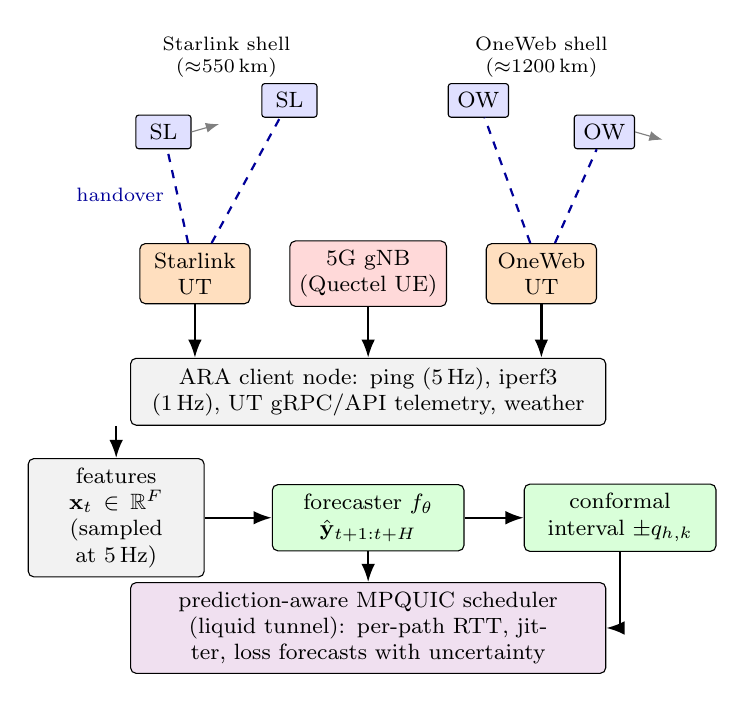
\begin{tikzpicture}[
  font=\footnotesize, >=Latex,
  sat/.style={draw, fill=blue!12, minimum width=7mm, minimum height=4mm, rounded corners=1pt},
  ut/.style={draw, fill=orange!25, minimum width=14mm, minimum height=6mm, align=center, rounded corners=2pt},
  blk/.style={draw, fill=gray!10, minimum height=7mm, align=center, rounded corners=2pt, text width=20mm},
  pred/.style={draw, fill=green!15, minimum height=7mm, align=center, rounded corners=2pt, text width=22mm},
  lnk/.style={->, thick},
  wl/.style={dashed, thick, blue!60!black}
]
% Satellites
\node[sat] (s1) at (0,4.2) {SL};
\node[sat] (s2) at (1.6,4.6) {SL};
\node[sat] (o1) at (4.0,4.6) {OW};
\node[sat] (o2) at (5.6,4.2) {OW};
\node[font=\scriptsize, align=center] at (0.8,5.15) {Starlink shell\\($\approx$550\,km)};
\node[font=\scriptsize, align=center] at (4.8,5.15) {OneWeb shell\\($\approx$1200\,km)};
\draw[->, gray] (s1.east) -- ++(0.35,0.1);
\draw[->, gray] (o2.east) -- ++(0.35,-0.1);
% UTs and gNB
\node[ut] (sut) at (0.4,2.4) {Starlink\\UT};
\node[ut] (out) at (4.8,2.4) {OneWeb\\UT};
\node[ut, fill=red!15] (gnb) at (2.6,2.4) {5G gNB\\(Quectel UE)};
\draw[wl] (sut) -- (s1); \draw[wl] (sut) -- (s2);
\draw[wl] (out) -- (o1); \draw[wl] (out) -- (o2);
\node[font=\scriptsize, blue!60!black] at (-0.55,3.4) {handover};
% Client node
\node[blk, text width=58mm, minimum height=8mm] (client) at (2.6,0.9) {ARA client node: ping (5\,Hz), iperf3 (1\,Hz), UT gRPC/API telemetry, weather};
\draw[lnk] (sut) -- (sut |- client.north);
\draw[lnk] (gnb) -- (client);
\draw[lnk] (out) -- (out |- client.north);
% Pipeline
\node[blk] (feat) at (-0.6,-0.7) {features $\mathbf{x}_t\in\mathbb{R}^{F}$\\(sampled at 5\,Hz)};
\node[pred] (model) at (2.6,-0.7) {forecaster $f_\theta$\\$\hat{\mathbf{y}}_{t+1:t+H}$};
\node[pred] (cp) at (5.8,-0.7) {conformal\\interval $\pm q_{h,k}$};
\draw[lnk] (client.south -| feat) -- (feat);
\draw[lnk] (feat) -- (model);
\draw[lnk] (model) -- (cp);
\node[blk, text width=58mm, fill=violet!12] (sched) at (2.6,-2.1) {prediction-aware MPQUIC scheduler (liquid tunnel): per-path RTT, jitter, loss forecasts with uncertainty};
\draw[lnk] (cp.south) |- (sched.east);
\draw[lnk] (model.south) -- (sched.north);
\end{tikzpicture}
}
  \caption{System model. Three access links are measured in parallel on the ARA client node. The forecaster maps a window of link-state features to a distribution of future RTT, jitter, and loss, which a conformal step turns into calibrated intervals for the prediction-aware MPQUIC scheduler.}
  \label{fig:system}
\end{figure}

\subsection{Forecasting problem and data}
For a link, let $\mathbf{x}_t\in\mathbb{R}^{F}$ be the feature vector at row $t$ and $\mathbf{y}_t\in\mathbb{R}^{K}$ the $K=3$ targets (RTT in ms, iperf jitter in ms, iperf loss in \%). Given the window $\mathbf{X}_t=(\mathbf{x}_{t-L+1},\dots,\mathbf{x}_t)$ with $L=30$ rows, the model predicts $\mathbf{y}_{t+h}$ for $h=1,\dots,H$ with $H=15$. The input covers 6\,s of history and the horizon spans 0.2\,s to 3\,s. Sessions (one CSV file each) are split 70/15/15 into training, validation, and test sets by a random permutation with seed 42, exactly as in the initial study. The test sessions are never seen during training, model selection, or calibration. Table~\ref{tab:data} lists the six datasets.

\begin{table}[htbp]
\centering
\caption{Datasets. Windows are 30 input rows plus 15 target rows at 5\,Hz. For 5G, every fourth training window is used. Features: initial set / final set.}
\label{tab:data}
\small
\begin{tabular}{lrrrrrr}
\toprule
Link & Sessions (tr/va/te) & Train windows & Val windows & Test windows & Features \\
\midrule
OneWeb DL   & 45 / 9 / 11   & 117{,}558 & 22{,}655  & 27{,}492  & 9 / 31 \\
OneWeb UL   & 45 / 9 / 11   & 115{,}847 & 22{,}751  & 28{,}125  & 9 / 31 \\
Starlink DL & 37 / 7 / 9    & 105{,}906 & 20{,}025  & 25{,}838  & 19 / 41 \\
Starlink UL & 37 / 7 / 9    & 106{,}165 & 20{,}090  & 25{,}666  & 19 / 41 \\
5G DL       & 266 / 57 / 58 & 194{,}725$^\dagger$ & 166{,}266 & 169{,}204 & 10 / 32 \\
5G UL       & 265 / 56 / 58 & 193{,}502$^\dagger$ & 162{,}894 & 168{,}519 & 10 / 32 \\
\bottomrule
\end{tabular}

\smallskip
\footnotesize $^\dagger$ after keeping every fourth window (778{,}898 and 774{,}006 before subsampling).
\end{table}


\section{Audit of the Previous Pipeline}
\label{sec:audit}
We rebuilt the initial evaluation in one script (\texttt{experiments/\allowbreak final\_benchmark.py}) that loads the data with the initial functions, uses the same session split, and trains the initial Seq2Seq-GRU with the initial optimizer settings. With the original data it reproduces the initial Starlink DL result (MAE \ReproSLMAE, RMSE \ReproSLRMSE, $R^2$ \ReproSLRtwo, against 8.55, 14.95, and 0.406 in the Modeling Dynamics report) and the OneWeb DL result (MAE \ReproOWMAE, RMSE \ReproOWRMSE, $R^2$ \ReproOWRtwo, against 6.12, 23.73, and 0.217). The script was then reviewed independently, and the surviving findings were fixed. Table~\ref{tab:audit} summarizes them.

\begin{table}[htbp]
\centering
\caption{Issues found in the previous pipeline and how this report handles them.}
\label{tab:audit}
\small
\begin{tabularx}{\linewidth}{>{\raggedright\arraybackslash}p{3.3cm}X>{\raggedright\arraybackslash}p{3.8cm}}
\toprule
Issue & Effect on initial numbers & Handling in this report \\
\midrule
A1. Horizon unit & Steps of 200\,ms were labeled as seconds. The ``15\,s'' horizon is 3\,s. & Horizons reported as $h\times 0.2$\,s. \\
A2. Interval coverage & Intervals were built from quantiles of the \emph{test} residuals, so PICP$_{95}$ is 0.95 by construction. & Conformal intervals calibrated on validation sessions, coverage measured on test sessions. \\
A3. Starlink RTT interpolation & Missing server pings are interpolated toward the \emph{next} real ping (\InterpFracSLDL\% of the DL and \InterpFracSLUL\% of the UL test targets). The last input row can contain part of the first target. & Inputs hold the last real ping for every method. Targets keep the measured series. \\
A4. Constant targets & OneWeb UL jitter and loss are zero in every row but were averaged into the aggregate with $R^2=1$. & $R^2$ undefined and left out of averages. \\
A5. ``Relative RMSE'' & Compared the model with a lag-1 shift of the flattened series, not with a persistence forecast. & Skill against persistence $\hat{y}_{t+h}=y_t$ per target and horizon. \\
A6. One seed & Each model was trained once. & Three seeds, seed ensembles, session-level bootstrap. \\
\bottomrule
\end{tabularx}
\end{table}

\paragraph{Effect of the leak.} Replacing the interpolated inputs raises the Starlink DL persistence RTT error at the first step by \AuditPersHonePct\%, from \AuditPersLegacyHone\,ms to \AuditPersCausalHone\,ms RMSE. To measure the effect on a trained forecaster, we trained the initial model (S2S) and the final model (DS2S) on Starlink DL with the interpolated and with the causal inputs, three seeds each, and tested the leaky models on both versions of the test inputs (Fig.~\ref{fig:leak}). Trained and tested on interpolated inputs, DS2S reports a 0.2\,s RTT MAE of \LeakDSAhOne\,ms. On the causal inputs that a deployed forecaster sees, the same model reaches \LeakDSBhOne\,ms, \LeakOptDSMAEhOne\% worse. The model trained on causal inputs reaches \LeakDSChOne\,ms, so causal training also gives the better deployed model. The gap shrinks with the horizon (\LeakOptDSMAEavg\% averaged over 0.2 to 3\,s) and is smaller for S2S (\LeakOptSSMAEhOne\% at 0.2\,s). The leak inflates exactly the short-horizon accuracy that a packet scheduler relies on most. Every result in this report uses causal inputs, and the initial model is retrained on them.

\begin{figure}[htbp]
  \centering
  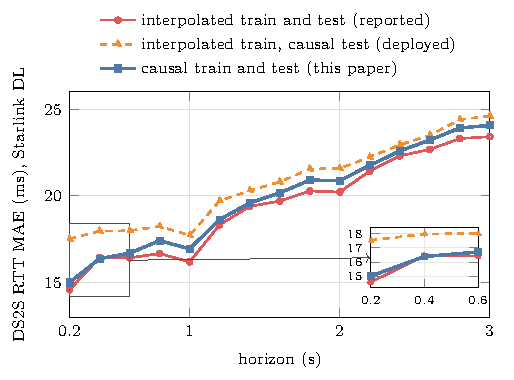
\includegraphics[width=0.85\linewidth]{figs_pdf/fr_leak.pdf}
  \caption{Effect of the interpolation leak on a trained forecaster (DS2S, Starlink DL, mean of three seeds). Trained and tested on interpolated inputs, the model reports a lower error than it reaches on the causal inputs available online. Inset: the first 0.6\,s.}
  \label{fig:leak}
\end{figure}

\paragraph{iperf alignment.} The iperf3 collector stamps each one-second report at the start of its interval, and the parsers snap it to the nearest ping row. An iperf value at row $t$ can therefore describe traffic up to about one second after $t$. The same alignment is used for every method and in the initial study. It is listed as an open problem in Section~\ref{sec:open}.


\section{What Is Predictable in Sub-Second Link State?}
\label{sec:predictable}
Before comparing forecasters, we ask which properties of the RTT carry over from the 6\,s input window to the 3\,s horizon. The statistics use the measured pings of the training sessions, each centered on its own mean, with session-bootstrap confidence intervals (script \texttt{fr\_volatility.py}).

\begin{figure}[htbp]
  \centering
  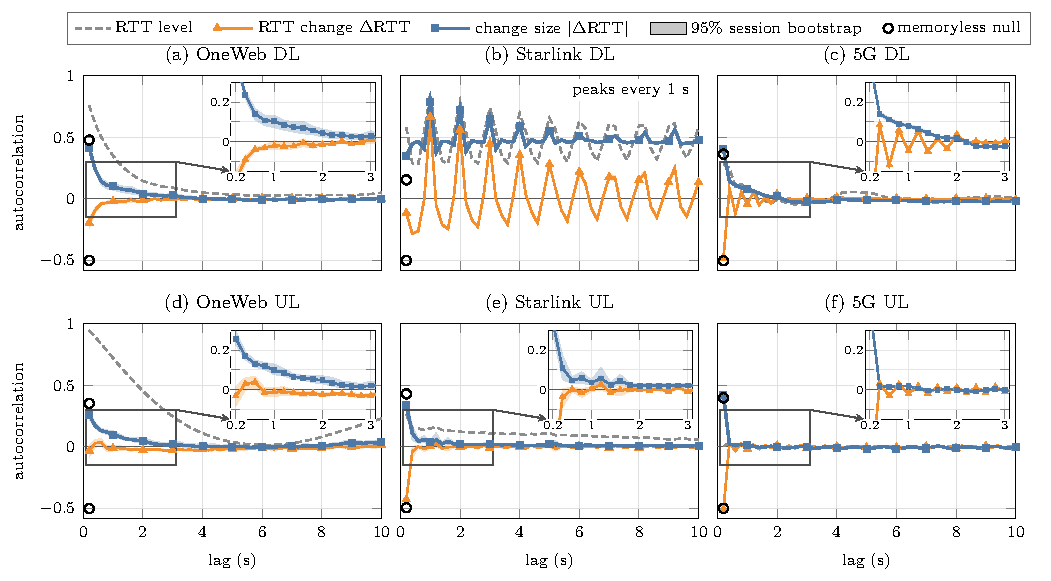
\includegraphics[width=\linewidth]{figs_pdf/fr_volatility.pdf}
  \caption{Autocorrelation of the RTT level, of its 200\,ms change $\Delta$RTT, and of the size of the change $|\Delta\mathrm{RTT}|$ in the training sessions (shaded: 95\% session-bootstrap interval). Circles: value of a memoryless series at 0.2\,s. Insets: lags of 0.2 to 3\,s. Starlink DL peaks every second because of a load-driven sawtooth.}
  \label{fig:vol}
\end{figure}

\paragraph{The next change is hard to predict, the level reverts.} From 0.4\,s to 10\,s the autocorrelation of $\Delta$RTT stays within $\pm$\VolDmaxAbs{} on five links (Fig.~\ref{fig:vol}). Past changes say almost nothing about the next change. The direction is still partly predictable because the RTT returns toward its recent level. Expecting a return to the mean of the input gets the sign of the 1\,s change right in \VolSignRevLo\% to \VolSignRevHi\% of the test windows (balanced accuracy), and the learned forecasters reach \VolSignNNLo\% to \VolSignNNHi\%. Point forecasts beat persistence mainly by not repeating the last, noisy ping. Their MAE is \PersRatioLo{} to \PersRatioHi{} times lower than that of persistence, but none of them gets much closer to the next value than the others, which is why the RMSE hardly separates them.

\paragraph{The spread depends on the link state.} On OneWeb and 5G, the SD of the 6\,s input does not predict the error of a 1\,s forecast within a session (rank correlation \VolWithinLo{} to \VolWithinHi), but it does between sessions (\VolBetweenLo{} to \VolBetweenHi). Each session runs in a noise regime set by its load and radio conditions, and a few seconds of input reveal it. Starlink DL is different. Under the saturating downlink test its RTT climbs from about 35\,ms to about 200\,ms in steps of about 50\,ms and drops back once per second. The sawtooth switches on and off within a session, and the volatility of the last 6\,s predicts that of the next 3\,s (within-session rank correlation \VolSLDLrv). We attribute it to queue build-up and drain under load, since the uplink test does not show it.

\paragraph{Errors are skewed upward.} Queues and retransmissions add delay, while nothing removes delay below the propagation floor. For the 1\,s forecasts of the initial model, the 97.5\% error quantile is \SkewQUL{} times the size of the 2.5\% quantile on 5G UL and \SkewOWDL{} times on OneWeb DL.

\paragraph{Consequence.} A constant-width interval around a point forecast, as in the previous report, ignores both properties. Calibrated to cover 95\% of all windows, it covers \CovConstCalmLo{} to \CovConstCalmHi{} of the calmest tenth and \CovConstVolLo{} to \CovConstVolHi{} of the most volatile tenth. Because the interval score is minimized by the conditional quantiles~\cite{gneiting2007strictly}, a forecaster should learn the spread and its skew from the input and be calibrated on sessions it has not seen. Fig.~\ref{fig:trace1min} shows the result on one minute of Starlink DL.

\begin{figure}[htbp]
  \centering
  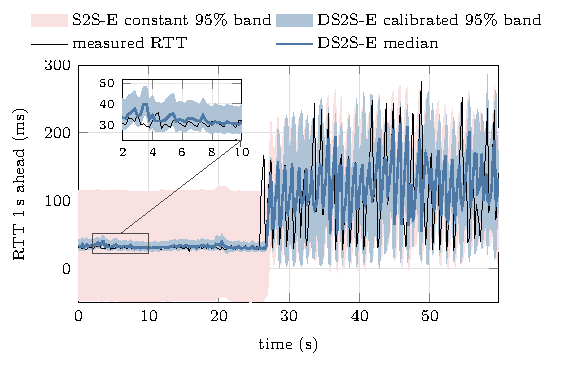
\includegraphics[width=0.95\linewidth]{figs_pdf/fr_trace.pdf}
  \caption{One minute of a Starlink DL test session, forecast 1\,s ahead. The initial model (S2S-E) has a constant 95\% interval of \TraceWidS\,ms. The calibrated interval of the final model (DS2S-E) is \TraceWidDCalm\,ms wide (median) while the link is quiet and \TraceWidDLoad\,ms once it swings. Inset: the quiet part.}
  \label{fig:trace1min}
\end{figure}


\section{The Final Forecaster}
\label{sec:methods}
The final forecaster (DS2S) keeps the encoder and attention of the initial Seq2Seq-GRU~\cite{cho2014learning,bahdanau2015neural} and changes it in four steps, each evaluated separately in Section~\ref{sec:results}. Figure~\ref{fig:arch} shows the result.

\begin{figure}[t]
  \centering
  \resizebox{0.8\linewidth}{!}{% final forecaster: GRU encoder, additive attention, residual autoregressive decoder.
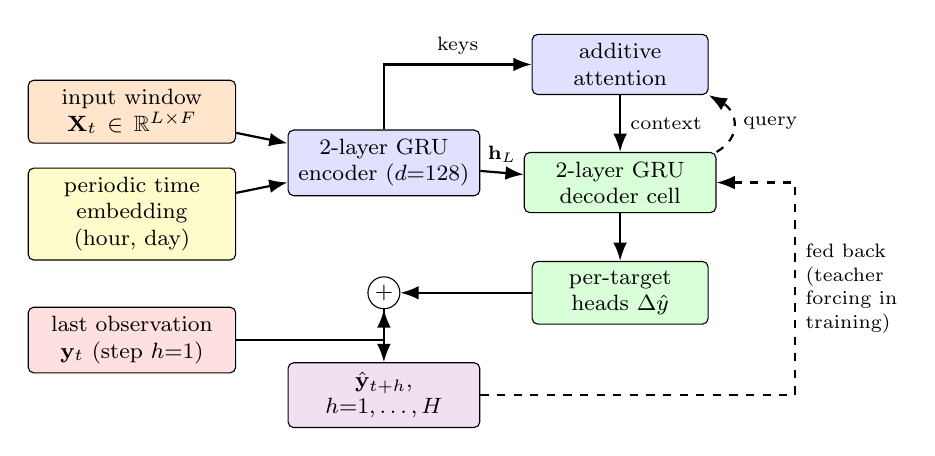
\begin{tikzpicture}[
  font=\footnotesize, >=Latex,
  b/.style={draw, rounded corners=2pt, minimum height=7mm, align=center, fill=#1},
  b/.default=gray!10,
  lnk/.style={->, thick}
]
\node[b=orange!20, text width=24mm] (in) at (0,0) {input window\\$\mathbf{X}_t\in\mathbb{R}^{L\times F}$};
\node[b=yellow!20, text width=24mm] (te) at (0,-1.3) {periodic time\\embedding (hour, day)};
\node[b=blue!12, text width=22mm] (enc) at (3.2,-0.65) {2-layer GRU\\encoder ($d{=}128$)};
\node[b=blue!12, text width=20mm] (att) at (6.2,0.6) {additive\\attention};
\node[b=green!15, text width=22mm] (dec) at (6.2,-0.9) {2-layer GRU\\decoder cell};
\node[b=green!15, text width=20mm] (head) at (6.2,-2.3) {per-target\\heads $\Delta\hat{y}$};
\node[draw, circle, inner sep=1pt, fill=white] (sum) at (3.2,-2.3) {$+$};
\node[b=red!12, text width=24mm] (last) at (0,-2.9) {last observation\\$\mathbf{y}_t$ (step $h{=}1$)};
\node[b=violet!12, text width=22mm] (out) at (3.2,-3.6) {$\hat{\mathbf{y}}_{t+h}$, $h{=}1,\dots,H$};
\draw[lnk] (in) -- (enc);
\draw[lnk] (te) -- (enc);
\draw[lnk] (enc) |- node[pos=0.75, above]{\scriptsize keys} (att);
\draw[lnk] (enc) -- node[above]{\scriptsize $\mathbf{h}_L$} (dec);
\draw[lnk] (att) -- node[right]{\scriptsize context} (dec);
\draw[lnk] (dec) -- (head);
\draw[lnk] (head) -- (sum);
\draw[lnk] (last) -| (sum);
\draw[lnk] (sum) -- (out);
\draw[lnk, dashed] (out.east) -| ++(4.0,0) |- node[pos=0.25, right, align=left]{\scriptsize fed back\\[-1pt]\scriptsize (teacher\\[-1pt]\scriptsize forcing in\\[-1pt]\scriptsize training)} (dec.east);
\draw[lnk, dashed] (dec.north east) to[out=30, in=-30, looseness=1.4] node[right]{\scriptsize query} (att.south east);
\end{tikzpicture}
}
  \caption{Final forecaster. The encoder and attention are those of the initial model. The decoder is anchored on the last observation and each head outputs a mean and five non-crossing quantiles of the change.}
  \label{fig:arch}
\end{figure}

\paragraph{Step 1: residual decoder.} The initial decoder starts from a zero vector and predicts each level directly. The final decoder starts from the last observed values and predicts the change,
\begin{equation}
\hat{\mathbf{y}}_{t+h} = \hat{\mathbf{y}}_{t+h-1} + g_\theta(\mathbf{s}_h), \qquad \hat{\mathbf{y}}_{t} = \mathbf{y}_t ,
\label{eq:resid}
\end{equation}
where $\mathbf{s}_h$ is the decoder state. With $g_\theta\equiv 0$ the model is the persistence forecast. Teacher forcing is applied per sample~\cite{bengio2015scheduled}.

\paragraph{Step 2: causal pipeline and context features.} Causal ping inputs (A3) for every method. Logger sentinels in the 5G radio values (for example SINR $=-32768$) are set to missing and forward filled. For each target we add seven causal per-session statistics (rows since the last change, mean and maximum over the last second, means over 30\,s and 60\,s, SD over 60\,s, and the session-to-date mean) and the time since the previous row. These give the model a view longer than its 6\,s window. Non-target inputs are clipped to $[-5,5]$ after $z$-scoring.

\paragraph{Step 3: distributional heads.} Link-state targets are heavy tailed. The RTT RMSE of the retrained initial model is \RatioRMSEMAEMin{} to \RatioRMSEMAEMax{} times its MAE, against about 1.25 for Gaussian errors. Squared-error training learns the conditional mean, which is not the best forecast under absolute error and says nothing about uncertainty~\cite{gneiting2011making}. Each head therefore outputs a mean $\hat{\mu}$ and the quantiles $\hat{q}_\tau$ for $\tau\in\mathcal{T}=\{0.025, 0.25, 0.5, 0.75, 0.975\}$, anchored as in~\eqref{eq:resid}. The quantiles are the median plus or minus cumulative softplus gaps, which rules out crossing. The loss on normalized targets is
\begin{equation}
\mathcal{L} = \frac{1}{NHK}\sum_{n,h,k}\Big[\big(\hat{\mu}_{nhk}-y_{nhk}\big)^2 + \frac{\omega}{|\mathcal{T}|}\sum_{\tau\in\mathcal{T}}\rho_\tau\big(y_{nhk}-\hat{q}_{\tau,nhk}\big)\Big],
\qquad \rho_\tau(e)=\max\{\tau e,(\tau-1)e\},
\label{eq:loss}
\end{equation}
with the pinball loss $\rho_\tau$~\cite{koenker1978regression} and weight $\omega=1$ in the main study. The mean is used for RMSE and $R^2$, the median for MAE. The model has \ParamsDist{} parameters against \ParamsResid{} for the Step 1 model on OneWeb DL.

\paragraph{Step 4: calibration and ensembles.} Quantiles learned on training sessions are not guaranteed to cover unseen sessions. We calibrate them with conformalized quantile regression (CQR)~\cite{romano2019conformalized}. For each target and step, the score on validation window $i$ is $s_i=\max\{\hat{q}_{0.025,i}-y_i,\ y_i-\hat{q}_{0.975,i}\}$, $c$ is its $\lceil (n+1)(1-\alpha)\rceil$-th smallest value, and the test interval is $[\hat{q}_{0.025}-c,\ \hat{q}_{0.975}+c]$ with $\alpha=0.05$. Models without quantiles get the split conformal interval $\hat{y}\pm q$~\cite{lei2018distribution}. Windows of one session are correlated and sessions differ in load, so the coverage guarantee is approximate~\cite{barber2023conformal}, and we report the coverage measured on the test sessions. The three seeds are averaged into a deep ensemble~\cite{lakshminarayanan2017simple} that is calibrated in the same way. Ensembles are marked ``-E'' (S2S-E for the initial model, DS2S-E for the final model).

\paragraph{References and comparison models.} Persistence ($\hat{\mathbf{y}}_{t+h}=\mathbf{y}_t$), a one-second seasonal repeat, and direct ridge regressions on the initial features (Ridge) and the final features (Ridge-E). To bound how specific the gain is to DS2S, we also train a linear quantile model (LQR), the final network with Gaussian heads (GS2S), and the final network with a scalar output (S2S-AE), all calibrated in the same way.

\paragraph{Training and metrics.} All neural models use the initial optimizer settings (AdamW, learning rate $10^{-3}$, weight decay $10^{-3}$, batch 512, hidden size 128) with a 60-epoch budget and early stopping after 15 epochs. All \NRuns{} runs stopped after \EpochsMin{} to \EpochsMax{} epochs with the selected checkpoint at or before epoch \BestEpochMax, so the budget does not limit the models. For 5G every fourth training window is used, for every method. We report MAE, RMSE, $R^2$, skill against persistence, the measured coverage (PICP) of the calibrated 95\% interval, and the interval score~\cite{gneiting2007strictly}
\begin{equation}
\mathrm{IS}_\alpha(l,u,y)=(u-l)+\tfrac{2}{\alpha}(l-y)\mathbb{1}\{y<l\}+\tfrac{2}{\alpha}(y-u)\mathbb{1}\{y>u\},
\end{equation}
called MIS in the Modeling Dynamics report. Lower is better. Per-target numbers are averages over the 15 steps.


\section{Results}
\label{sec:results}
All results are on the test sessions. ``Initial'' is the initial Seq2Seq-GRU retrained on the corrected data with the same protocol as the final model.

\subsection{Headline: RTT with session-level uncertainty}
The test windows of one session overlap and share its regime, so the unit of independent evidence is the session. Table~\ref{tab:boot} and Fig.~\ref{fig:bootstrap} compare the two ensembles with a paired bootstrap over whole test sessions (2000 replicates, script \texttt{fr\_bootstrap.py}). The interval score improves significantly on all six links, and DS2S-E has the lower interval score in each of the \BSnSessTot{} test sessions. The MAE improves significantly on five links and is inconclusive on OneWeb UL. The RMSE improves significantly on Starlink DL and both 5G links and is inconclusive on the other three. No change is significantly worse. Coverage is close to 0.95 everywhere except Starlink UL, where both models under-cover slightly.

\begin{table}[htbp]
\centering
\caption{RTT on the test sessions, averaged over 0.2--3\,s, for the three-seed ensembles S2S-E (initial) and DS2S-E (final). Changes with 95\% session-bootstrap intervals. Bold: the interval excludes zero. MAE uses the median of DS2S-E, RMSE the means. IS and PICP refer to the calibrated 95\% interval.}
\label{tab:boot}
\resizebox{\linewidth}{!}{%
\begin{tabular}{l rrr rrr rrr cc}
\toprule
 & \multicolumn{3}{c}{Interval score (ms)} & \multicolumn{3}{c}{MAE (ms)} & \multicolumn{3}{c}{RMSE (ms)} & \multicolumn{2}{c}{PICP} \\
\cmidrule(lr){2-4}\cmidrule(lr){5-7}\cmidrule(lr){8-10}\cmidrule(lr){11-12}
Link & S2S-E & DS2S-E & $\Delta$\% [95\% CI] & S2S-E & DS2S-E & $\Delta$\% [95\% CI] & S2S-E & DS2S-E & $\Delta$\% [95\% CI] & S2S-E & DS2S-E \\
\midrule
\tabinput{data/tab_main_boot.tex}
\bottomrule
\end{tabular}}
\end{table}

\begin{figure}[htbp]
  \centering
  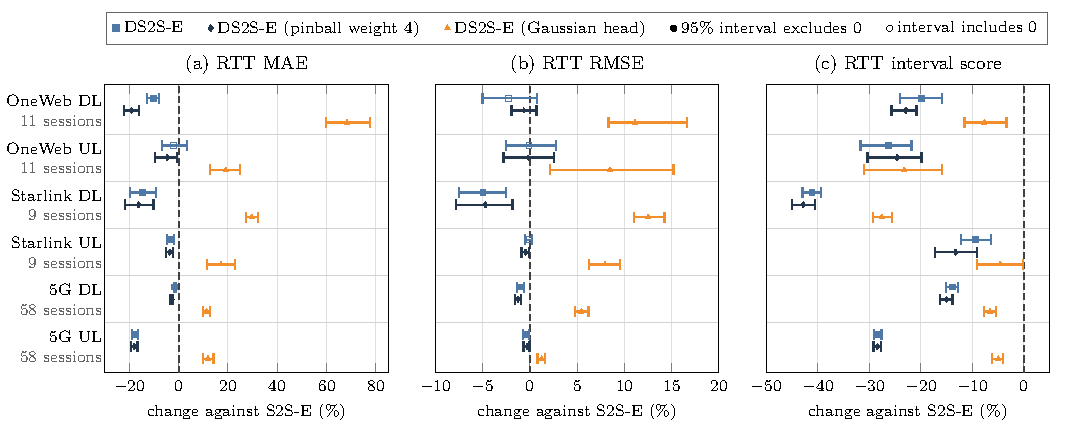
\includegraphics[width=\linewidth]{figs_pdf/fr_bootstrap.pdf}
  \caption{Session-level bootstrap of the RTT change of DS2S-E against S2S-E (2000 replicates). Marker: bootstrap median. Bar: 95\% percentile interval. Filled: the interval excludes zero. Negative values favor DS2S-E.}
  \label{fig:bootstrap}
\end{figure}

A bootstrap over windows would give intervals \BSWidRatioLo{} to \BSWidRatioHi{} times narrower and would call two inconclusive changes significant. Leaving out any one test session moves the interval-score change by at most \BSLooMax{} points. A Wilcoxon test over sessions confirms the MAE gain at the 1\% level on five links (the final model wins \SessWinsTotal{} of \SessNTotal{} sessions). Table~\ref{tab:main} adds the seed spread of the single models, and Fig.~\ref{fig:hzoom} shows the errors per horizon.

\begin{table}[htbp]
\centering
\caption{RTT results on the test sessions, averaged over the 15 steps (0.2--3\,s). Mean $\pm$ standard deviation over 3 seeds, and 3-seed ensembles. MAE, RMSE, and MIS in ms. MIS is the calibrated 95\% interval score (split conformal for Initial, CQR for Final).}
\label{tab:main}
\scriptsize
\setlength{\tabcolsep}{3pt}
\begin{tabular}{llccccc}
\toprule
Link & Model & MAE & RMSE & $R^2$ & MIS & PICP \\
\midrule
\tabinput{data/tab_main.tex}
\bottomrule
\end{tabular}
\end{table}

\begin{figure}[htbp]
  \centering
  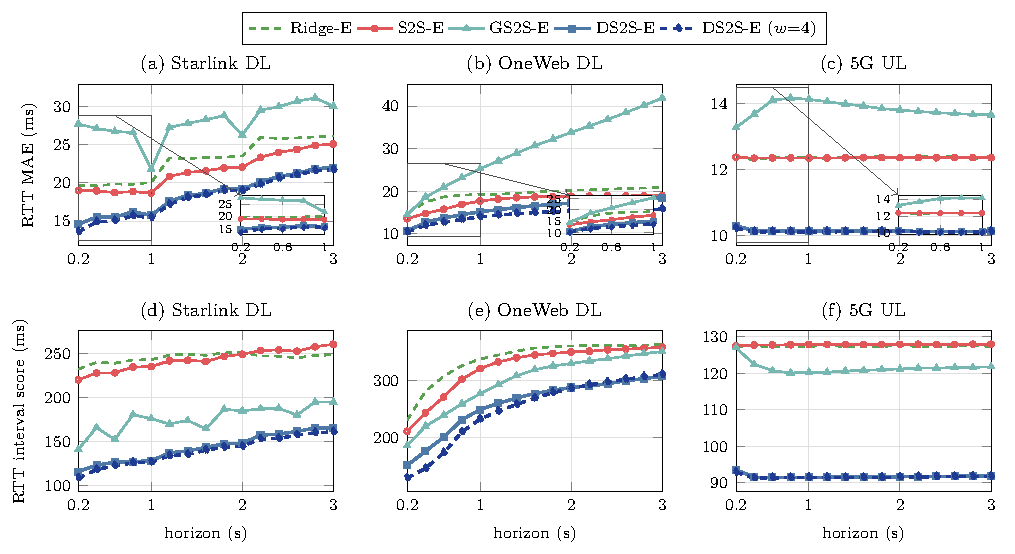
\includegraphics[width=\linewidth]{figs_pdf/fr_hzoom.pdf}
  \caption{RTT MAE (top) and calibrated 95\% interval score (bottom) per horizon on three links. DS2S-E ($w{=}4$) is the final model with pinball weight 4 (Section~\ref{sec:robust}). Insets: 0.2 to 1\,s.}
  \label{fig:hzoom}
\end{figure}

\subsection{Comparison with the Modeling Dynamics report}
Table~\ref{tab:isproto} shows why the previous evaluation could not see this gain. With intervals from the quantiles of the test residuals, the method of the previous report, the two models are within about 2\% of each other on every link, because both intervals then have a constant width. With intervals calibrated on held-out sessions, the final model changes the interval score by \ChgMISWorst\% to \ChgMISBest\% (seed means). Table~\ref{tab:y2} gives the previous ``aggregate'' (mean over the three targets and 15 steps) next to the printed numbers. The retrained initial model matches the MAE and RMSE of the Modeling Dynamics report closely. The $R^2$ differs on OneWeb UL because of A4 and on Starlink DL because the causal inputs remove the leaked signal (A3).

\begin{table}[htbp]
\centering
\caption{RTT interval score (ms, seed means) with the earlier method (test-residual quantiles around the mean) and with intervals calibrated on validation sessions.}
\label{tab:isproto}
\small
\begin{tabular}{lrrrrrr}
\toprule
 & \multicolumn{3}{c}{Earlier method} & \multicolumn{3}{c}{Calibrated} \\
\cmidrule(lr){2-4}\cmidrule(lr){5-7}
Link & Initial & Final & $\Delta$\% & Initial & Final & $\Delta$\% \\
\midrule
\tabinput{data/tab_isproto.tex}
\bottomrule
\end{tabular}
\end{table}

\begin{table}[htbp]
\centering
\caption{Aggregate in the style of the Modeling Dynamics report (mean over RTT, jitter, and loss and over the 15 steps). MIS (Initial method) uses quantiles of the test residuals. MIS (calibrated) uses intervals calibrated on validation sessions.}
\label{tab:y2}
\scriptsize
\begin{tabular}{llccccc}
\toprule
Link & Source & MAE & RMSE & $R^2$ & MIS (Initial method) & MIS (calibrated) \\
\midrule
\tabinput{data/tab_y2compare.tex}
\bottomrule
\end{tabular}
\end{table}

\subsection{Which step helps?}
Table~\ref{tab:ablation} adds the final steps one at a time. The residual decoder (Step 1) and the causal pipeline with context features (Step 2) do not improve the MAE. On OneWeb DL they make it worse, because a squared-error model anchored on a spiky last value follows the spikes. Step 2 lowers the RMSE slightly on most links (up to 4.5\% on Starlink DL). The gains in MAE and interval score come from Step 3, the distributional heads. The ensemble (Step 4) adds up to 6.4 further points (Starlink DL MAE).

\begin{table}[htbp]
\centering
\caption{Ablation: change (\%) of RTT MAE, RMSE, and calibrated interval score (MIS) relative to the retrained initial model (seed means, the last row compares the final ensemble with the initial seed mean). Negative is better.}
\label{tab:ablation}
\scriptsize
\setlength{\tabcolsep}{2pt}
\resizebox{\linewidth}{!}{%
\begin{tabular}{l*{18}{r}}
\toprule
 & \multicolumn{3}{c}{OneWeb DL} & \multicolumn{3}{c}{OneWeb UL} & \multicolumn{3}{c}{Starlink DL} & \multicolumn{3}{c}{Starlink UL} & \multicolumn{3}{c}{5G DL} & \multicolumn{3}{c}{5G UL} \\
\cmidrule(lr){2-4}\cmidrule(lr){5-7}\cmidrule(lr){8-10}\cmidrule(lr){11-13}\cmidrule(lr){14-16}\cmidrule(lr){17-19}
Steps & MAE & RMSE & MIS & MAE & RMSE & MIS & MAE & RMSE & MIS & MAE & RMSE & MIS & MAE & RMSE & MIS & MAE & RMSE & MIS \\
\midrule
\tabinput{data/tab_ablation.tex}
\bottomrule
\end{tabular}}
\end{table}

\subsection{Simple references}
Table~\ref{tab:baselines} adds the references that the initial study did not have. Persistence is a poor RTT forecast at 5\,Hz because single pings are noisy. A tuned linear model on the final features (Ridge-E) is within one point of the initial network on RMSE skill on four links. On Starlink DL a repeat of the value one second earlier already has 28\% skill, which reflects the one-second sawtooth. The final ensemble has the lowest MAE and the highest skill on every link (tied on 5G UL). Ridge on the initial features fails on 5G UL because of unclipped logger sentinels.

\begin{table}[htbp]
\centering
\caption{RTT MAE (ms) and RMSE skill against persistence (\%, higher is better) for the references and the neural models (seed means).}
\label{tab:baselines}
\scriptsize
\setlength{\tabcolsep}{3pt}
\begin{tabular}{l*{12}{r}}
\toprule
 & \multicolumn{2}{c}{OneWeb DL} & \multicolumn{2}{c}{OneWeb UL} & \multicolumn{2}{c}{Starlink DL} & \multicolumn{2}{c}{Starlink UL} & \multicolumn{2}{c}{5G DL} & \multicolumn{2}{c}{5G UL} \\
\cmidrule(lr){2-3}\cmidrule(lr){4-5}\cmidrule(lr){6-7}\cmidrule(lr){8-9}\cmidrule(lr){10-11}\cmidrule(lr){12-13}
Method & MAE & skill & MAE & skill & MAE & skill & MAE & skill & MAE & skill & MAE & skill \\
\midrule
\tabinput{data/tab_baselines.tex}
\bottomrule
\end{tabular}
\end{table}

\subsection{Jitter and loss}
Table~\ref{tab:targets} gives the jitter and loss results. Point accuracy is similar for both models, with exceptions in both directions. The calibrated interval scores of the final model are lower on every link and target, often by a large factor (Starlink DL jitter: 2.8 against 8.5). Jitter and loss are one-second iperf reports with long runs of zeros and rare large values, the case where input-dependent intervals help most.

\begin{table}[htbp]
\centering
\caption{Jitter (ms) and loss (\%) on the test sessions (seed means, OneWeb UL omitted because both are zero in every row).}
\label{tab:targets}
\scriptsize
\begin{tabular}{llcccccc}
\toprule
 & & \multicolumn{3}{c}{Jitter} & \multicolumn{3}{c}{Loss} \\
\cmidrule(lr){3-5}\cmidrule(lr){6-8}
Link & Model & MAE & RMSE & MIS & MAE & RMSE & MIS \\
\midrule
\tabinput{data/tab_targets.tex}
\bottomrule
\end{tabular}
\end{table}


\section{Why the Interval Improves}
\label{sec:why}
\paragraph{The gain is in the interval, at every horizon.} Fig.~\ref{fig:heat} shows the change of the RTT MAE and interval score of DS2S-E against S2S-E for every link and step. The interval score improves in every cell, most at short horizons on the satellite links. Almost all of the MAE gain comes from reporting the median instead of the mean. On the five links other than Starlink DL, the mean of DS2S-E changes the MAE by \MeanMAELo\% to $+$\MeanMAEHi\%, against \MedMAELo\% to \MedMAEHi\% for its median. Starlink DL is the one link where the mean also improves (\MeanMAESLDL\%), because its sawtooth is partly predictable.

\begin{figure}[t]
  \centering
  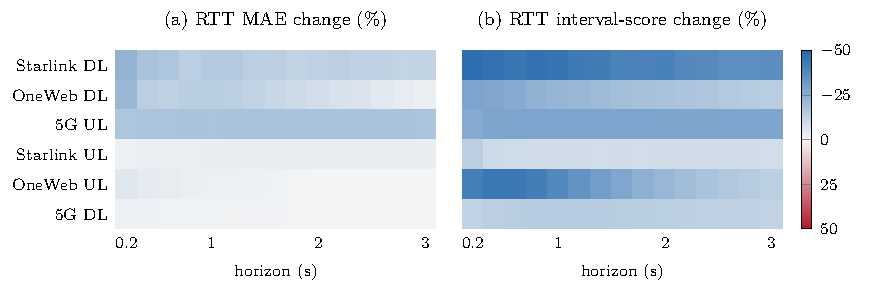
\includegraphics[width=0.85\linewidth]{figs_pdf/fr_heat.pdf}
  \caption{Change (\%) of the RTT MAE and of the calibrated 95\% interval score of DS2S-E against S2S-E per link and horizon step. Blue: DS2S-E is better.}
  \label{fig:heat}
\end{figure}

\paragraph{Conditional coverage.} Fig.~\ref{fig:condcov} breaks the coverage down by the volatility of the input window (deciles of the input RTT SD) and by horizon. The constant interval of S2S-E over-covers quiet windows and under-covers volatile ones. On Starlink DL it covers the calmest tenth at \CovConstSLDLdOne{} and the most volatile tenth at \CovConstSLDLdTen. Scaling the interval with the input SD reverses the error, because the future error grows much more slowly than the input SD. The largest decile deviation from 0.95 (coverage gap) of DS2S-E is \GapDSSLDL{} on Starlink DL, \GapDSQDL{} on 5G DL, and \GapDSQUL{} on 5G UL, against \GapConstSLDL{}, \GapConstQDL{}, and \GapConstQUL{} for the constant interval. The reduction is significant on these three links and on Starlink UL. On OneWeb it is not. DS2S-E widens its interval only \WidRatioOWDL{} times (DL) and \WidRatioOWUL{} times (UL) from the calmest to the most volatile tenth, while the error grows \ErrRatioOWDL{} and \ErrRatioOWUL{} times, and it covers that tenth only at \CovDSOWDLdTen{} and \CovDSOWULdTen. An SD-scaled interval with a tuned floor covers it at \CovNormTunedOWDLdTen{} and \CovNormTunedOWULdTen, so the input carries the warning and DS2S-E under-reacts to it.

\begin{figure}[t]
  \centering
  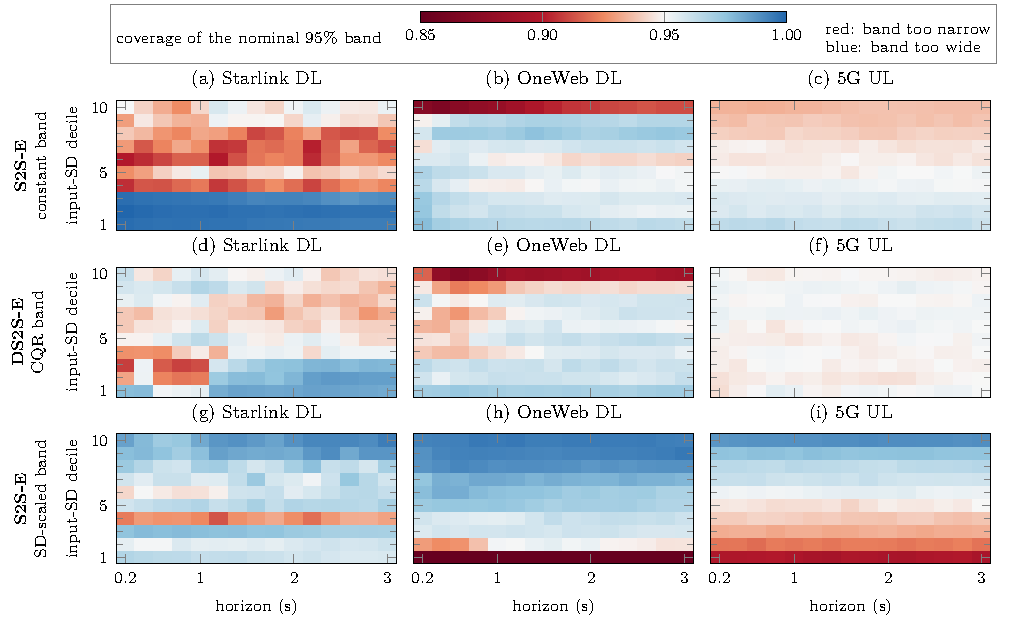
\includegraphics[width=\linewidth]{figs_pdf/fr_condcov.pdf}
  \caption{Conditional coverage of the calibrated 95\% RTT intervals on the test sessions per input-SD decile and horizon step. White: nominal 0.95. Blue: wider than needed. Red: too narrow (below 0.85 shares the darkest red). Bottom row: interval scaled by the input SD with a small floor.}
  \label{fig:condcov}
\end{figure}

\paragraph{Where the interval-score gain comes from.} We built intermediate intervals that change one ingredient at a time, all calibrated on the same sessions. Moving a constant interval from the S2S-E mean to the DS2S-E mean changes the score by \DecCentreLo\% to $+$\DecCentreHi\%, so the better center is not the source. Giving the S2S-E forecast the per-window width of DS2S-E, placed symmetrically, gains \DecWidthLoAbs\% to \DecWidthHiAbs\%. Placing it asymmetrically, as DS2S-E does, gains another \DecAsymLoAbs\% to \DecAsymHiAbs\%. The adaptive width carries most of the gain on Starlink DL and OneWeb UL, the skew on 5G UL.

\paragraph{How specific is the gain to the final model?} Table~\ref{tab:extent} lists every interval a deployed system could use. No interval around the S2S-E point forecast comes close to the quantile forecasters. The best of them is still \ExtBestPointLoAbs\% to \ExtBestPointHiAbs\% worse than DS2S-E on every link. The new inputs and decoder alone do not explain the gain either. S2S-AE-E shares them but outputs a mean, and it changes the interval score of S2S-E by only \ExtFrfullLo\% to $+$\ExtFrfullHi\%. \GaussSentence{} The linear quantile model LQR is within \ExtLQRMaxAbs\% of DS2S-E on every link and better on OneWeb UL and Starlink UL. DS2S-E is significantly better only on \LQRsigLinks, by \LQRsigLo\% to \LQRsigHi\%. The source of the gain is therefore the distributional output calibrated across sessions, which a linear model can exploit too. What the recurrent network adds is a better point forecast: against LQR it lowers the RMSE on all six links (\LQRRMSELoAbs\% to \LQRRMSEHiAbs\%, all significant).

\begin{table}[t]
\centering
\caption{Interval score (IS, ms) and coverage gap over input-SD deciles of the 95\% RTT intervals on the test sessions. SD-scaled: floor tuned on the calibration sessions. S2S-AE-E: inputs and decoder of DS2S-E with a scalar output. Bold: lowest IS of the link. GS2S-E \GaussSeedNote.}
\label{tab:extent}
\resizebox{\linewidth}{!}{%
\begin{tabular}{ll*{12}{r}}
\toprule
 & & \multicolumn{2}{c}{OneWeb DL} & \multicolumn{2}{c}{OneWeb UL} & \multicolumn{2}{c}{Starlink DL} & \multicolumn{2}{c}{Starlink UL} & \multicolumn{2}{c}{5G DL} & \multicolumn{2}{c}{5G UL} \\
\cmidrule(lr){3-4}\cmidrule(lr){5-6}\cmidrule(lr){7-8}\cmidrule(lr){9-10}\cmidrule(lr){11-12}\cmidrule(lr){13-14}
Forecast & Interval & IS & gap & IS & gap & IS & gap & IS & gap & IS & gap & IS & gap \\
\midrule
\tabinput{data/tab_extent.tex}
\bottomrule
\end{tabular}}
\end{table}


\section{Robustness of the Gain}
\label{sec:robust}
\subsection{Sensitivity to the design choices}
Each alternative setting was trained with two seeds on the four satellite links (80 additional runs, \texttt{results\_final/sweeps/}): a 3\,s and a 12\,s input window, a 6\,s horizon, hidden sizes 64 and 256, and pinball weights $\omega=0.25$ and $\omega=4$ in~\eqref{eq:loss}. Table~\ref{tab:sweepvs} compares the final and initial models trained with the same setting. The interval-score gain holds in every setting and on every link, from 7\% to 41\%, and so does the MAE gain. The RMSE changes by $-7.8\%$ to $+2.1\%$. The conclusions therefore do not depend on the window or horizon chosen in the initial study.

\begin{table}[t]
\centering
\caption{Change (\%) of the final model against the initial model trained with the same setting (RTT, two seeds, averaged over all steps of the setting). Negative is better.}
\label{tab:sweepvs}
\scriptsize
\setlength{\tabcolsep}{2.5pt}
\begin{tabular}{l*{12}{r}}
\toprule
 & \multicolumn{3}{c}{OneWeb DL} & \multicolumn{3}{c}{OneWeb UL} & \multicolumn{3}{c}{Starlink DL} & \multicolumn{3}{c}{Starlink UL} \\
\cmidrule(lr){2-4}\cmidrule(lr){5-7}\cmidrule(lr){8-10}\cmidrule(lr){11-13}
Setting & MAE & RMSE & MIS & MAE & RMSE & MIS & MAE & RMSE & MIS & MAE & RMSE & MIS \\
\midrule
\tabinput{data/tab3_sweeps_vs.tex}
\bottomrule
\end{tabular}
\end{table}

For the final model itself (scored on the same 0.2--3\,s targets in every setting):
\begin{itemize}[leftmargin=*]
  \item \textbf{Input window.} A 12\,s window helps OneWeb UL (MAE $-9.4\%$) and hurts OneWeb DL ($+11.2\%$). A per-link window is an easy gain.
  \item \textbf{Horizon.} Training for 6\,s costs little at 0.2--3\,s on three links but raises the Starlink DL MAE by 7.8\%. The interval score of the final model stays below that of the initial model at every step up to 6\,s.
  \item \textbf{Model size.} A hidden size of 64 is worse on the downlinks (up to $+7.9\%$ MAE). A size of 256 changes the results by a few percent in both directions.
  \item \textbf{Pinball weight.} \WeightSentence{} The main results with $\omega=1$ therefore understate what the distributional model can reach (Fig.~\ref{fig:hzoom}).
\end{itemize}

\subsection{Adaptivity, handovers, and training cost}
The width of the final 95\% RTT interval is positively rank-correlated with the absolute error on every link (\RhoMin{} to \RhoMax), highest on Starlink DL and OneWeb, where the RTT alternates between calm periods and bursts. Table~\ref{tab:events} splits the test windows by whether a satellite handover occurs inside the 3\,s horizon. On OneWeb UL a handover more than doubles the RTT error of both models, and neither anticipates it. Elsewhere the errors around handovers are similar to the errors outside, and the final gain is of the same size in both groups. Handover flags alone do not predict the RTT jumps. A full forecast takes \TimeDSCPU\,ms on one CPU thread against \TimeSSCPU\,ms for the initial model, well below the 200\,ms between measurements.

\begin{table}[t]
\centering
\caption{RTT MAE (ms) of the ensembles for test windows with and without a handover inside the forecast horizon.}
\label{tab:events}
\small
\setlength{\tabcolsep}{4pt}
\begin{tabular}{lrrrrrrr}
\toprule
 & & \multicolumn{3}{c}{handover in horizon} & \multicolumn{3}{c}{no handover} \\
\cmidrule(lr){3-5}\cmidrule(lr){6-8}
Link & windows (\%) & Initial & Final & $\Delta$\% & Initial & Final & $\Delta$\% \\
\midrule
\tabinput{data/tab2_events.tex}
\bottomrule
\end{tabular}
\end{table}

\subsection{What the model uses}
Input gradients and attention weights of DS2S (seed 0, 20{,}000 test windows per link, \texttt{fr\_attention.py}) tell different stories. The forecast is most sensitive to the newest second of input, which receives \GradLastLo\% to \GradLastHi\% of the input gradient (17\% if uniform), and \GradEngLo\% to \GradEngHi\% of the sensitivity at the 3\,s step goes to the engineered 30--60\,s and session statistics, which let the model read the session regime. The attention mostly looks elsewhere. On OneWeb and 5G UL it puts \AttnSinkLo\% to \AttnSinkHi\% of its weight on the oldest encoder state, and on Starlink UL and 5G DL it is nearly flat. Replacing it with a fixed map or uniform weights raises the RTT MAE by at most \AttnAblMax\% on Starlink and 5G and by $+$\AttnAblOWDL\% on OneWeb DL. The gain of DS2S comes from its distributional output and its inputs, not from where it attends.


\section{Value for Prediction-Aware Multipath Scheduling}
\label{sec:sched}
The initial QoE-predictive scheduler uses point forecasts of each path. The calibrated upper bound $\hat{q}_{0.975}+c$ of the final model is a per-path, per-step RTT bound that holds about 95\% of the time on unseen sessions. Because it depends on the input, it is tight when a path is stable and loose only when the path is about to burst. A constant-width bound is equally wide at all times. This section measures what that difference is worth (script \texttt{fr\_scheduler.py}).

\paragraph{Emulation.} We emulate deadline-aware packet duplication on the test sessions of the four satellite links, with the satellite path as primary and the 5G path of the same direction as backup. At time $t$ the scheduler plans the packets it will send at $t+h$, $h\in\{0.2,\dots,3\}$\,s. A packet on the primary misses its deadline $D$ if the measured RTT at $t+h$ exceeds $D$, set to the 90th percentile of the calibration-session RTT (\SchedDSLDL\,ms on Starlink DL). The scheduler duplicates a packet on the backup when its forecast bound exceeds $D$. We count the share of duplicated packets, which costs backup capacity, and the share of late packets that were not duplicated (misses).

\begin{figure}[htbp]
  \centering
  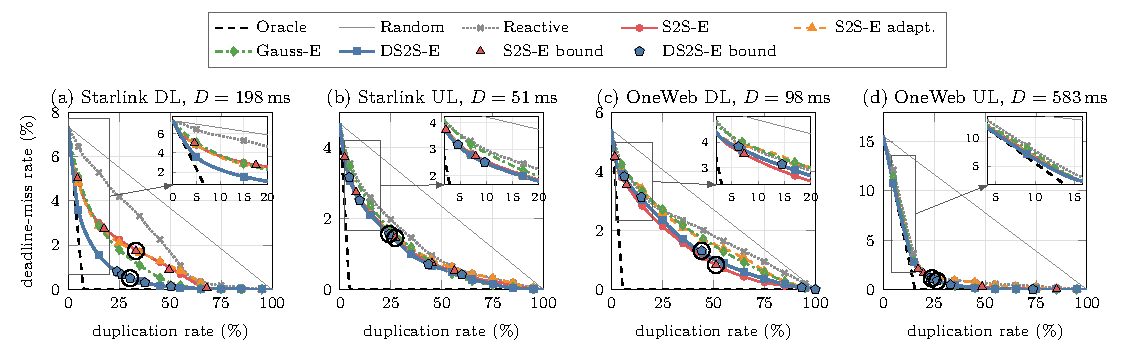
\includegraphics[width=\linewidth]{figs_pdf/fr_scheduler.pdf}
  \caption{Deadline-aware duplication on the test sessions: share of late, non-duplicated packets against the share of duplicated packets, pooled over 0.2--3\,s. Curves sweep the knob of each policy. Markers: one-sided bounds calibrated at 0.80 to 0.99, circled at 0.95. Insets: low duplication. S2S-E adapt.\ scales its margin by the input volatility.}
  \label{fig:sched}
\end{figure}

\paragraph{Deployable comparison.} A deployed scheduler must set its knob in advance. For S2S-E we use the one-sided 95\% conformal upper bound. For DS2S-E we set the knob on the calibration sessions so that its miss rate there equals that of the S2S-E bound. On Starlink DL, the S2S-E bound duplicates \SchedSSdupSLDL\% of the packets and misses \SchedSSmissSLDL\%. DS2S-E duplicates \SchedDSdupSLDL\% and misses \SchedDSmissSLDL\%, which is \SchedSaveSLDL\% less duplication (95\% CI \SchedSaveSLDLlo{} to \SchedSaveSLDLhi\%) with no more misses. On Starlink UL and OneWeb UL the two schedulers tie (duplication change \SchedSaveSLUL\% and \SchedSaveOWUL\%). On OneWeb DL, DS2S-E needs \SchedDSdupCurveOWDL\% duplication to reach the miss rate of the S2S-E bound, which duplicates \SchedSSdupOWDL\%. Every forecaster with the anchored decoder loses there, including the point forecaster S2S-AE-E, so the loss comes from the decoder and not from the distributional output. The same decoder ranks the rare OneWeb DL spikes worse (AUROC \AUCFROWDL{} against \AUCPrevOWDL{} for the initial model), while on Starlink DL it is the best spike warning (\AUCFRSLDL{} against \AUCPrevSLDL).

\paragraph{Where the gain comes from.} At the miss rate of the S2S-E bound on Starlink DL, S2S-AE-E needs \SchedFFdupSLDL\% duplication, DS2S-E \SchedDSdupCurveSLDL\%, and S2S-E \SchedSSdupCurveSLDL\%. About half of the gain comes from the new inputs and decoder and half from the predictive distribution. \GaussSchedSentence{} The saving is largest for deadlines between the 90th and 97.5th percentile and at short lead times. It shrinks for the 99th percentile, which lies beyond the 97.5\% quantile that DS2S-E describes.

\paragraph{Same mean, different risk.} Fig.~\ref{fig:risk} groups the test windows by the S2S-E mean forecast and, within each group, by the spread that DS2S-E predicts. At the same mean forecast of \RiskMeanLo{} to \RiskMeanHi\,ms on Starlink DL, \RiskLowPct\% of the packets are late when DS2S-E predicts a narrow spread and \RiskHighPct\% when it predicts a wide one. A scheduler that sees only the mean must treat these windows alike.

\begin{figure}[htbp]
  \centering
  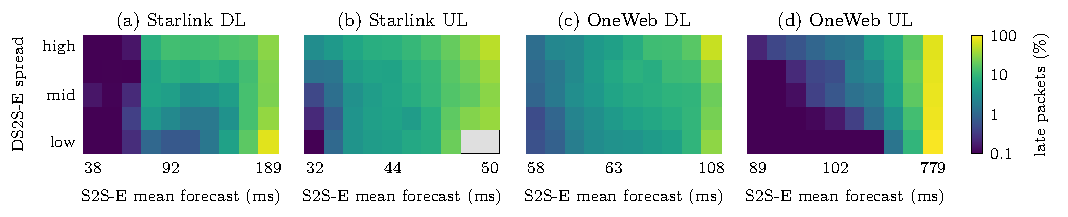
\includegraphics[width=\linewidth]{figs_pdf/fr_scheduler_risk.pdf}
  \caption{Same mean, different risk. Share of late packets (log color scale) when the test windows are grouped by the S2S-E mean forecast (deciles, x) and, within each decile, by the predicted DS2S-E spread $\hat{q}_{0.975}-\hat{q}_{0.5}$ (quintiles, y).}
  \label{fig:risk}
\end{figure}

\paragraph{Caveats.} Only the bound-against-bound comparison is deployable. The curves sweep each knob on the test windows, like an ROC curve. On the test sessions the one-sided 95\% bounds covered \BoundCovLo{} to \BoundCovHi{} of the RTT values. The satellite and 5G sessions were not recorded at the same time, so the emulation assumes independent paths. If they are, the 5G UL backup itself exceeds the Starlink UL deadline in \BackupQULSL\% of its samples, which raises the DS2S-E miss rate on Starlink UL from \BackupDSmissSLUL\% to \BackupDSmissCorrSLUL\%.


\section{Open Questions, Open Problems, and How to Close the Gaps}
\label{sec:open}
This section is new. It collects what the final work did not settle, separates questions we cannot yet answer from problems we know how to attack, and gives a plan to close each gap. Table~\ref{tab:gaps} is the summary. Each row names the evidence in this report, the work that would close the gap, and the measurement that would show it is closed.

\begin{table}[t]
\centering
\caption{Open gaps, the evidence for each, how to close it, and when it counts as closed. Effort: S (days, existing data and code), M (weeks, new training or code), L (a new measurement campaign or system test).}
\label{tab:gaps}
\footnotesize
\begin{tabularx}{\linewidth}{>{\raggedright\arraybackslash}p{2.6cm}>{\raggedright\arraybackslash}X>{\raggedright\arraybackslash}X>{\raggedright\arraybackslash}p{3.0cm}c}
\toprule
Gap & Evidence & How to close it & Closed when & Effort \\
\midrule
G1. RTT level not predictable & RMSE within \BSRMSEMaxAbs\% of the initial model on every link. $\Delta$RTT has almost no memory (Section~\ref{sec:predictable}). & Add information the 6\,s window lacks: the Starlink 15\,s reallocation slots~\cite{tanveer2023making}, the state of the other paths, terminal telemetry at a higher rate. & RTT RMSE skill rises by more than the seed spread on two or more links. & M \\
G2. Volatile OneWeb windows under-covered & DS2S-E covers the most volatile tenth at \CovDSOWDLdTen{} (DL) and \CovDSOWULdTen{} (UL), an SD-scaled interval at \CovNormTunedOWDLdTen{} and \CovNormTunedOWULdTen{} (Section~\ref{sec:why}). & Regime-conditional calibration: conformal offsets per input-volatility bin, or a CQR interval with an SD-scaled floor. & Coverage gap on OneWeb below that of the constant interval with no worse interval score. & S \\
G3. OneWeb DL spikes and duplication & Spike AUROC \AUCFROWDL{} against \AUCPrevOWDL. More duplication than the initial bound (Section~\ref{sec:sched}). & Anchor the decoder on a robust recent level (median of the last second) or gate between anchored and free decoding. & DS2S-E at least ties S2S-E in the OneWeb DL emulation. & M \\
G4. Calibration under session shift & Starlink UL coverage 0.930 to 0.936 for every interval. Validation sessions serve both early stopping and calibration. & Separate calibration sessions from early-stopping sessions. Online adaptive conformal correction during operation~\cite{gibbs2021adaptive}. & Test coverage within $\pm0.01$ of 0.95 on every link, also in a later campaign. & S \\
G5. Tails beyond the 97.5\% quantile & Duplication saving shrinks for deadlines at the 99th percentile (Section~\ref{sec:sched}). & Add the 0.99 and 0.995 quantiles to the heads and calibrate them. & Saving at the 99th percentile deadline comparable to that at the 95th. & S \\
G6. Pinball weight not tuned & $\omega=4$ is preferred on all six links (Section~\ref{sec:robust}). & Retrain the main study with $\omega=4$ and rerun all analyses. & Main tables reported with the tuned weight. & S \\
G7. iperf time stamps & Reports are stamped at the start of their one-second interval (Section~\ref{sec:audit}). & Re-stamp at the end of the interval in the parsers and rerun. & Jitter and loss inputs strictly causal. Results change by less than the seed spread, or the change is reported. & S \\
G8. One campaign, one split & Sessions from one campaign per link, one random session split, 5G training subsampled. & Time-ordered splits (train on earlier, test on later sessions), several splits, full 5G training set. & Gains hold on sessions recorded after the training data. & M \\
G9. Scheduler gain only emulated & Paths not recorded at the same time. Emulation assumes independent paths and a saturating test load (Section~\ref{sec:sched}). & Simultaneous recording of all paths under realistic traffic. End-to-end test of the final model in the liquid tunnel. & Fewer late frames or less duplicated traffic in the tunnel at equal QoE. & L \\
\bottomrule
\end{tabularx}
\end{table}

\subsection{Open questions}
These are questions the data of this project cannot answer yet.
\begin{itemize}[leftmargin=*]
  \item \textbf{Is the RTT level predictable with more information (G1)?} Section~\ref{sec:predictable} shows that the next change is close to unpredictable from the last 6\,s of the same path. It does not show that it is unpredictable from information outside that window. The Starlink reallocation every 15\,s is scheduled and globally synchronized, so its timing is knowable in advance. The state of the other paths may reveal shared causes such as local load. A longer window helped OneWeb UL and hurt OneWeb DL, so more history alone is not the answer.
  \item \textbf{Is the Starlink DL sawtooth a property of the link or of the test?} The one-second sawtooth appears only under the saturating downlink iperf test and is the most predictable structure in the data. Under the real traffic of the multipath client the queue may not build up in this way, and part of the Starlink DL gain may not carry over. Recording under realistic traffic (G9) answers this.
  \item \textbf{Do the results transfer to other times, terminals, and places (G8)?} Each link was measured in one campaign with one terminal at one site. Both the regime structure and the calibration offsets may change with season, firmware, and constellation growth. Only new data can test this.
  \item \textbf{How much of the emulated gain survives end to end (G9)?} The emulation counts late and duplicated packets. The client cares about frames and QoE, and duplication interacts with congestion control and with the capacity of the backup path.
  \item \textbf{When is the network worth it?} LQR recovers most of the interval gain. DS2S-E adds a better point forecast and a better scheduler result on Starlink DL. Whether that is worth the larger model depends on the target hardware and on the end-to-end result.
\end{itemize}

\subsection{Open problems}
These are known shortcomings with a clear path to a fix.
\begin{itemize}[leftmargin=*]
  \item \textbf{OneWeb under-reaction (G2).} The input carries the warning that DS2S-E ignores. An SD-scaled interval with a tuned floor covers the most volatile OneWeb tenth almost at the nominal level. Calibrating the final quantiles separately per volatility bin, or taking the wider of the CQR interval and an SD-scaled floor, uses this information without retraining.
  \item \textbf{Anchored decoder on spiky links (G3).} Anchoring on the last value helps where the RTT moves smoothly and hurts where single spikes are followed by a return to the base level. The fix is to anchor on a robust recent level, or to let the model learn a gate between the anchored and the free decoder per link.
  \item \textbf{Calibration and shift (G4).} The validation sessions are used for early stopping and for calibration. Splitting them, or using cross-conformal calibration, removes the dependence. For drift in operation, an online adaptive conformal update adjusts the offset after each observed miss and keeps the long-run coverage at the target.
  \item \textbf{Strict deadlines (G5).} The heads describe the distribution only up to the 97.5\% quantile, and the conformal offset extrapolates beyond it. Adding upper quantiles is a small change to the heads and the loss.
  \item \textbf{Settings and pipeline (G6, G7).} The pinball weight and the iperf stamps are one-line changes followed by a full rerun, which takes about seven hours with the scripts of Appendix~\ref{app:repro}.
\end{itemize}

\subsection{Plan to close the gaps}
We propose three stages, ordered so that each stage uses only data and code that the previous one provides.
\begin{enumerate}[leftmargin=*]
  \item \textbf{Consolidate (weeks 1 to 4, existing data).} Fix the iperf stamps (G7), retrain with $\omega=4$ and two extra upper quantiles (G5, G6), split calibration from early stopping (G4), and add regime-conditional calibration (G2). Rerun every table, figure, and number with the existing scripts. Report the change of each fix against this report.
  \item \textbf{Improve the forecaster (weeks 4 to 10, existing data).} Test the robust anchor and the gated decoder on OneWeb DL (G3). Add the Starlink slot timing and cross-path features (G1). Accept a change only if it improves the interval score or the RMSE beyond the seed spread with the session bootstrap of Section~\ref{sec:results}. Compare the final candidate with LQR at equal calibration to decide the deployed model.
  \item \textbf{Validate in the system (from week 8, new data).} Record all paths at the same time on ARA under the traffic of the multipath client, in sessions spread over several weeks (G8, G9). Test the forecasters trained on the existing data on the new sessions without retraining, then with online calibration. Run the final model inside the liquid tunnel and compare late frames and duplicated traffic with the minRTT scheduler and with the initial predictive scheduler.
\end{enumerate}
The first stage needs no new measurements and can start immediately. The third stage is the only one that tests the claim that matters most for the project, that calibrated forecasts improve multipath delivery.


\appendix
\section{Reproducing the Results}
\label{app:repro}
All code is in \texttt{modeling/} of the project repository. The commands below regenerate every number, table, and figure. They take about seven hours on an Apple M3 Max with six jobs in parallel. \texttt{docs/final\_report/REPRODUCE.md} lists the analysis scripts (\texttt{fr\_*.py}) behind each figure.

\begin{small}
\begin{verbatim}
cd modeling
# all 78 jobs (link, method, seed), 5G uses --train_stride 4
cat results_final/main/jobs.txt | xargs -P 6 -L 1 results_final/main/run_job.sh
# tables, ensembles and figure data
python3 experiments/final_aggregate.py && python3 experiments/final_extras.py
python3 experiments/final_audit_numbers.py && python3 experiments/final_tables.py
# figures of the report (from reports/final_report)
python3 build_figs.py
\end{verbatim}
\end{small}

\noindent Main files: \texttt{experiments/final\_benchmark.py} (data loading on the initial split, training, baselines, metrics, conformal calibration), \texttt{models/seq2seq\_dist.py} (the final forecaster), \texttt{dataset.py} (causal ping fix, sentinel cleaning, context features, input clipping), \texttt{results\_final/main/<link>/} (per-run metrics, settings, trained models), and \texttt{results\_final/summary/} (summaries, per-horizon values for all 15 steps, and the deployment CQR offsets).


\bibliographystyle{IEEEtran}
\bibliography{refs}

\end{document}
